\documentclass[a4paper,12pt]{article}

\usepackage{mathrsfs,amsthm,graphicx,bm,amssymb,enumerate}
\usepackage{amsmath}
\usepackage{mathrsfs}
\usepackage{txfonts}
\usepackage{mathtools}
\usepackage{empheq}
\usepackage[symbol]{footmisc}
\usepackage{mathrsfs}
\usepackage{enumitem}
\usepackage{xpatch}
\usepackage{caption}
\usepackage{secdot}

%~ \usepackage[]{titlesec}%
%~ \titleformat{\subsubsec}
%~ {\Large\bfseries}
%~ {\ul{\thesubsubsec.\enspace}}
%~ {-0.15em}
%~ {\ul}



\renewcommand{\thefootnote}{\arabic{footnote}}


\DeclareMathOperator{\x}{\mathrm{X}}
\DeclareMathOperator{\la}{\mathrm{L}}
\DeclareMathOperator{\ka}{\mathrm{K}}
\DeclareMathOperator{\md}{\mathrm{mod}}

\theoremstyle{definition}
{\newtheoremstyle{underlinethm}% name
{-1.5mm}        % Space above, empty = `usual value'
{}              % Space below
{}              % Body font
{}    % Indent amount (empty = no indent, \parindent = para indent)
{\bfseries}              % Thm head font
{}             % Punctuation after thm head
{1.5mm}         % Space after thm head: \newline = linebreak
{{{\thmname{#1}\thmnumber{ #2}~\thmnote{(#3)}}}}

\theoremstyle{underlinethm}
\newtheorem{thm}{Theorem}[section]
\newtheorem{example}{Example}[section]
\newtheorem{definition}{Definition}[section]
\newtheoremstyle{underline}% name
{-1.5mm}        % Space above, empty = `usual value'
{}              % Space below
{}              % Body font
{}    % Indent amount (empty = no indent, \parindent = para indent)
{\bfseries}              % Thm head font
{}             % Punctuation after thm head
{1.5mm}         % Space after thm head: \newline = linebreak
{{{\thmname{#1}{\underline{(\thmnumber{ #2})}\relax}~\thmnote{(#3)}}}}  % Thm head spec

\theoremstyle{definition}
\newtheorem{subsubsec}{}[subsection]





%~ \theoremstyle{definition}


%~ \newtheorem{theorem}{Theorem}[section]
%~ \newtheorem{subsubsec}{}[subsection]

%~ \newtheorem{innercustomgeneric}{\customgenericname}
%~ \providecommand{\customgenericname}{}
%~ \newcommand{\newcustomtheorem}[2]{%
  %~ \newenvironment{#1}[1]
  %~ {%
   %~ \renewcommand\customgenericname{#2}%
   %~ \renewcommand\theinnercustomgeneric{##1}%
   %~ \innercustomgeneric
  %~ }
  %~ {\endinnercustomgeneric}
%~ }

%~ \newcustomtheorem{customthm}{Theorem}


\usepackage{tikz}
\usetikzlibrary{calc}
\newcommand*{\vertchar}[2][0pt]{%
  \tikz[
    inner sep=0pt,
    shorten >=-.15ex,
    shorten <=-.15ex,
    line cap=round,
    baseline=(c.base),
  ]\draw
    (0,0) node (c) {#2}
    ($(c.south)+(#1,0)$) -- ($(c.north)+(#1,0)$);%
}


\renewcommand{\thesection}{\arabic{section}}

\makeatother

\begin{document}

\title{Polynomial Representation of Quantum Entanglement Properties of Resonating Valence Bond States and Related States}
\author{Sudipto Singha Roy\footnote{Sudipto will fill in as he is abroad}, Aditi Sen(De){\footnote{Harish-Chandra Research Institute, Chatnag Road, Jhusi, Allahabad, 211019, India.}}, Ujjwal Sen{$^\dagger$} and\\ Ajit Iqbal Singh{\footnote{The Indian National Science Academy, Bahadeirshah Zafar Marg, New Delhi, 110002, India.}}}

\date{\today}

\maketitle

\section*{Abstract}

We study quantum entanglement properties of Resonating valence bond states and related states via polynomial representation. This renders easy proofs of genuine entanglemnet of doped states as well.


\section{Introduction}\label{section-1}

Resonating Valence Bond states (RVB) are important in condensed matter physics. Phillip W. Anderson's RVB paper [A1] is perhaps the most important paper that triggered intensive and extensive studies of the topic. The progress from physics point of view can be gauged by survey or history articles by Anderson [A2 and A3], Baskaran [Ba 1, Ba 2], Poilblanc, Cirac \& Perez-Garaia [PCPG], Shuch [Sh], Zaanen [Z] and an enormous collection of papers cited in them or elsewhere. Some particular aspects concerning quantum entanglement for different types have been studied by Chandran, Kaszlikowski, Sen(De), Sen \& Vedral [CKSSV], Dhar \& Sen(De) [DS], Dhar, Sen(De) \& Sen[DSS], Roy, Dhar, Sen(De) \& Sen [RDSS] and Roy [R].


Polynomial have been used in different ways to study quantum entanglement. For instance, one can see papers by Wallach[W], Parthasarathy[P], Bhat[Bh],\break Skowronek[Sk], Sengupta, Arvind \& Singh [SAS], Josza \& Mitchinson[JM],\break Adesso \& Regula[Ad], Mor[M]. A recent paper by Bandyopadhyay \& Singh[BS] displays a simple way to use polynomials for understanding multipartite entanglement in general and Schmidt rank in particular cases. For multi-qubit systems, the\break theory of polynomial representation of quantum entanglement takes rather a\break simple form. Further, for RVB's and related states it is enough to confine attention to homogeneous polynomials. So we recast a part of [BS] and strengthen it further in Section~\ref{section-2}. The basic theory of polynomials required for this can be found in many standard books but as in [BS] we take Fulton[F] as our basic reference. Similarly for multipartite  entanglement we may refer to any standard source such as Horodecki's[HHH] and Szalay[Sz]. We confine our attention to pure states.

In Section~\ref{section-2}, we give polynomial representation of quantum entanglement by for a multiqubit system. It renders easy conditions for classification of a pure state into a product vector, product vector in a bipartite cut or genuinely entangled in terms of the degree, support, number of terms or irreducibility  of the corresponding polynomial.   

We began Section~\ref{section-3} with basics like coverings and resonating valence to the Cororings and resonance Valence bond states, nearest neighbour (in short, NN) coverings etc. together with a few examples for the sake of self-completeness. Then we give their polynomial representations and obtain results on conditions in terms of them for quantum entanglement properties of RVB states. This brings us to the notion of decomposability  and factorability  etc. for converings together with interrelationships amongst them and renders easy proof of the fact that NN RVB's are genuinely entangled. Master Equations are obtained in terms of coverings for the corresponding RVB state to be a product vector in some bipartite cut. Illustrations have been provided. Doped RVB states are genuinely entangled is shown to be true in a very easy way. Section~\ref{section-4} concentrates on variable coefficients analogues and differences as compared to the constant ones in Section~\ref{section-3}. Doped states with variable coefficient with non-zero sum are shown to be genuinely entangled by a short proof.


\section{Polynomial representation of quantum\\ entanglement for multi-qubit systems}\label{section-2}

Let $\mathbb{N}$ be the set of natural nuumbers $1,2,3, \ldots$ For $m\in \mathbb{N}$, let $\Gamma_{m}= \left\{ j \in \mathbb{N} : j \leq m \right\}$. For any set S, let $P_{S}$ be the set of subsets of S and $\#$ S, the cordinality of S.

We take empty sums to be zero and empty products to be 1.

Let $n \in \mathbb{N}$ with $n \geq 2$.

\subsection{Basics of multi-qubit systems and polynomials}\label{subsection-2.1}

We begin with qubit systems. Let $l \leq j \leq n.$ 

%~ \subsubsection*{(\underline{2.1.1})}
\begin{subsubsec}\label{subsubsection-2.1.1}
Let $\mathcal{H}_{j}$ be a qubit system with ordered basis $\left\{ | \uparrow \rangle_{j}, | \downarrow \rangle_{j}\right\}$ or $\left\{ | O \rangle_{j}, 1 \shortmid \rangle_{j}\right\}$ or $\left\{ \beta^{j}_{1}, \beta^{j}_{2} \right\}$ of orthonormal vectors.
\end{subsubsec}

%~ \subsubsection*{(\underline{2.1.2})}
\begin{subsubsec}\label{subsubsection-2.1.2}
We also consider $\mathcal{H}_{j}$ as the space $\vertchar[.08ex]{C}_{1}[\x_{j}]$ of complex polynomials in $\x_{j}$ of degree at most 
in place of root one, and the constant function $\bold{1}$ and the polynomial $\x_{j}$ constituting an orthonormal basis for $\mathcal{H}_{j}$.

In other words, we consider $\mathcal{H}_{j}$ as the subspace spanned by $\bold{1}$ and $\x_{j}$ of the Hilbert space $\la^{2}(T)$ of square Lebesgue integrable complex functions $f$ on the unit circle. i.e; torus T with $<f, g> = \int \bar{f} g d \lambda$, $\lambda$  being the normalized Lebesgue. measure on T.

\end{subsubsec}

%~ \subsubsection*{(\underline{2.1.3})}
\begin{subsubsec}\label{subsubsection-2.1.3}
Let $\mathcal{H} = \bigotimes\limits_{\rm d=1}^{\rm n} \mathcal{H}_{j}$ be the Hilbert space tensor product of Hilbert spaces $\mathcal{H}_{j}$, $1 \leq j \leq n$.

Let $\mathcal{I}$ be the set of n-tuples $\bold{i} = (i_{j})^{n}_{j=1}$ with $i_{j}=0$ or 1 for $1 \leq j \leq n$. Then $\mathcal{I}$ is in one-one correspondence with the set $P_{n}$ of subsets of $\Gamma_{n}$ via $\bold{i} \longrightarrow K_{\bold{i}} = \left\{j : i_{j} = 1 \right\}$. We note that for $o \leq s \leq n $, $\mathcal{I}_{s} = \left\{ \bold{i} \in \mathcal{I} : |\bold{i}| = \sum_{i=1}^{\rm n} i_{j} = s
\right\}$ equals $\left\{\bold{i} \in g : \# K_{\bold{i}} = s \right\}$ and together, they constitute a decomposition of $\mathcal{I}$.

Further, $\left\{| \bold{i} \rangle = \bigotimes\limits_{j=1}^{\rm n} : |\bold{i}_{j} = {({i_{j}})_{j=1}^{n}} \in \mathcal{I} \right\}$  is an orthonormal  basis for $\mathcal{H}$. A generic element $\xi$ of $\mathcal{H}$ has the form $\xi$ = $\sum_{\bold{i}\in \mathcal{I}} a_{\bold{i}} |\bold{i} \rangle$ for a unique $\bold{a} = {(a_{\bold{i}})_{\bold{i}\in \mathcal{I}}} \vertchar[.08ex]{C}^{\mathcal{I}}$.
\end{subsubsec}

%~ \subsubsection*{(\underline{2.1.4})}
\begin{subsubsec}\label{subsubsection-2.1.4}

Continuing in the spirit set in (2.1.2) above, for $\bold{i} \in \mathcal{I}$ 

\noindent
let $\bold{\x}^{\bold{i}} = \prod\limits_{j=1}^{n} \x_{j}^{i_{j}} = \prod \left\{ \x_{j} : j \in K_{\bold{i}} \right\} = \bold{\x}^{K_{\bold{i}}}$, so as to say by $\bold{\x}$ by $\bold{\x}^{\bold{i}}$ and accordingly, $\xi in \mathcal{H}$ as in (2.1.3) above, by the polynomial F in several variables $\x = (\x_{j})^{n}_{j=1} = (\x_{1}, \x_{2}, \ldots \x_{n})$ given by ${\rm F} (\bold{\x}) = \sum_{\bold{i}\in \mathcal{I}} a_{\bold{i}} \bold{\x}^{\bold{i}}$. This enables us to identity $\mathcal{H}$ with the space $\vertchar[.08ex]{C}_{1}[\bold{\x}]$ of polynomials F in $\bold{\x}$ with degree of each variable $\x_{j}$ being less than or equal to 1. Clearly the degree of each such F is at most $n$. We may also write F as $\sum\limits_{\rm K \in P_{n}} a_{\rm K} \bold{\x}^{\ka} = \sum\limits_{\rm K \in P_{n}} a_{\bold{i}_{\ka}} \bold{\x}^{\bold{i}_{K}}$, where for $\ka \in P_{n} (\bold{i}_{\ka})_{j} =1$ for $j\in \ka $ and $0$ otherwise.

In other words, we consider $\mathcal{H}$ as the subspace spanned by $\left\{ \bold{\x}^{\ka}, \ka \in P_{n}\right\}$ of the Hilbert space $\rm L^{2} \left(T^{n}\right)$ of square integrable complex functions $f$ on the torus $T^{n}$ with the normalized product Lebesque measure $\lambda_{n}$ and take $<f, g> = \int\limits_{T^{n}} \overline{f} g d \lambda_{n}$.
 
 \end{subsubsec}
 
%~ \subsubsection*{(\underline{2.1.5})} 
 \begin{subsubsec}\label{subsubsection-2.1.5}
 Consider any non-empty subset $E$ of $\Gamma_{n}$ with $E \neq \Gamma_{n}$. Let $E' = \Gamma_{n}\smallsetminus E = \{ j \in \Gamma_{n} : j \notin E \}$. Set $\mathcal{H}(E) = \bigotimes\limits_{j \in E} \mathcal{H}_{j}$ and $\mathcal{H}(E') = \bigotimes\limits_{j \in E'}$ $\mathcal{H}_{j}$.
 
 Then $\mathcal{H} = \mathcal{H}(E) \bigotimes \mathcal{H}(E')$ a two-fold tensor product in the bipartite cut $(E, E')$, so as to say.
 
 Let $\vertchar[.08ex]{C}_{1}[\bold{\x}_{E}]$ and  $\vertchar[.08ex]{C}_{1}[\bold{\x}_{E'}]$ have their obvious meanings. Further, $\vertchar[.08ex]{C}_{1}[\bold{\x}] = \vertchar[.08ex]{C}_{1}[\bold{\x}_{E}] \bigotimes  \vertchar[.08ex]{C}_{1}[\bold{\x}_{E'}]$. We note that for $p \in \vertchar[.08ex]{C}_{1}[\bold{\x}_{E}]$, $q \in \vertchar[.08ex]{C}_{1}[\bold{\x}_{E'}]$, $F = p \bigotimes q$ is given by $F(\bold{x}) = p (\bold{\x}_{E}) q (\bold{\x}_{E'})$.
 
 In view of (2.1.4) above we may identiy $\mathcal{H}(E)$ with $\vertchar[.08ex]{C}_{1}[\bold{\x}_{E}]$ and $\mathcal{H}(E')$ with $\vertchar[.08ex]{C}_{1}[\bold{\x}_{E'}]$.
 
 \end{subsubsec}
 
 %~ \subsubsection*{(\underline{2.1.6})}
 \begin{subsubsec}\label{subsubsection-2.1.6}
 Caution is needed in above identification because the context is important. For instance, for $n=4$, $E = \{ 1, 2 \}$, consider the polynomials written in the usual short form $1, \x_{1}-\x_{2}$.
 
 Means $10 \rangle_{1}$ in $\mathcal{H}_{1}$, $100\rangle_{12} = 10 \rangle_{1} \otimes 10 \rangle_{2}$ in $\mathcal(E)$, $100 \rangle_{34} = 10\rangle_{3} \otimes 10 \rangle_{4}$ in $\mathcal{H}(E')$ and $10000\rangle_{1234} = 10 \rangle_{1} \otimes 10 \rangle_{2} \otimes 10 \rangle_{3} \otimes 10 \rangle_{4}$ in $\mathcal{H}$. On the other hand, $X_{1}-X_{2}$ has no meaning in $\mathcal{H}_{1}$ or $\mathcal{H}(E')$ but it stands for $110\rangle_{12} - 101\rangle_{12} = 11 \rangle_{1} \otimes 10 \rangle_{2} - 10 \rangle_{1} \otimes 11 \rangle_{2}$ in $\mathcal{H}_{E}$ and for $11000 \rangle_{1234} - 10100\rangle_{1234} = 11 \rangle_{1} \otimes 10 \rangle_{2} \otimes 10 \rangle_{3} \otimes 10 \rangle_{4}-10 \rangle_{1} \otimes 10 \rangle_{2} \otimes 10 \rangle_{3} \otimes 10 \rangle_{4} $ in $\mathcal{H}$.
\end{subsubsec} 
 
 %%%%%%%%%%%%%%%%%%%%%%%%%%%%%%%%%%%%%%%%%%%%%page no 9 $$$$$$$$$$$$$$$$$$$$$$$$$$$$$$$$$$$$$$$$$$$$$$$$$$$$$$$
 
 \subsection{Multiqubit Entanglement and Polynomial Representation}\label{subsection-2.2}
 
 Let $0 \neq \xi  \in \mathcal{H}$ and $\digamma (\bold{\x})$, the corresponding polynomial in $\vertchar[.08ex]{C}_{1}[\bold{\x}]$. Set $P_{???} = \frac{1}{|| \xi||^{2}} | \xi\rangle \langle \xi|$, the corresponding pure state; i.e; the rank one (orthogonal) projection on the linear span of $\xi$. We consider the following concepts related to entanglement of $\xi$ or $P_{\xi}$ to being with. 
 
 %~ \subsubsection*{(\underline{2.2.1})}\label{2.2.1}
 
 \begin{subsubsec}\label{subsubsection-2.2.1}
 
 \begin{enumerate}[label=(\alph*)]
 \item $\xi$ is a product vector in $\mathcal{H} = \bigotimes\limits_{\rm n}^{j=1} \mathcal{H}_{j}$ if $\xi =\bigotimes\limits_{\rm n}^{j = 1} \xi_{j}$ with $\xi_{j} \in \mathcal{H}_{j}$ for $1 \leq j \leq n$. Otherwise, $\xi$ is called entangled vector.
   
 \item Let $\phi \neq E_{\neq} \subset \Gamma_{n}$ $\xi$ is said to be a product vector in the bipartite cut $(E, E')$ if $\xi$ is a product vector in $\mathcal{H}(E)\otimes \mathcal{H}(E')$, i.e; if $\xi = n \otimes 3$ for some $n \in \mathcal{H}(E)$ and $\xi \in \mathcal(E')$
 
 \item $\xi$ is said to be genuinely entangled if it is not product vector in any bipartite cut.
  
 \end{enumerate}
 
 Clearly for $n = 2$, $\xi$ is entangled if and only if $\xi$ is genuinely entangled.
 
 \end{subsubsec}
 
 %~ \subsubsection*{(\underline{2.2.2})}\label{subsubsection-2.2.2}
 
 \begin{subsubsec}\label{subsubsection-2.2.2}
 The concepts and properties above will be transferred to the corresponding $F(\bold{\x})$ i.e; $F$.
 
 We give some easy consequences as a Theorem below.
 
 We shall use the following notation and terminology for that.
 \end{subsubsec}
 
 \begin{enumerate}[label=(\alph*)]
 
 \item  Let $S_{F}$, the support of $F =\left\{ j \in \Gamma_{n} \; ; \x_{j}\;\; \text{occurs in} F, \text{i.e;}  F \text{has degree 1 in} \x_{j} \right\}$ and $m = \neq S_{F}$, the number of $\x_{j}'$s that occur in $F$.
 
 \item Let $d$ be the degree of $F$. Then $d > 0$ if and only if $m > 0$. Also $m \geq d$ simply because $F$ has degree at most one in each $\x_{j}$.
 
 \item $F$ is said to be homogeneous if each term in $F$ has degree $d$.  
 
 \item Suppose that $F = gh$ with $g$ and $h$ in $\vertchar[.08ex]{C}_{1} [\bold{\x}]$. Then $S_{g} \cap S_{h} = \emptyset$ because degree of $\x_{j}$ in $F(\bold{\x})$ is at most one for $1 \leq j \leq n$. If $g$ and $h$ are such that $S_{g} \neq \Gamma_{n} \neq S_{h}$ then we may take any $E$ with $\emptyset \neq E_{\neq}\subset \Gamma_{n}$ with $S_{g} \subset E$ and $S_{h} \subset E'$. This permits us to write $g(\x)$ as $g(\bold{\x}_{E})$ and $h(\bold{\x})$ as $h(\bold{\x}_{E'})$ as well and then $F(\underline{x}) = g(\x_{E}) h (\bold{\x}_{E'})$.
 
 \item By Problem 1.1 $[F]$ if $F, g, h$ are as in $(d)$ above and $F$ is homogeneous then so are $g$ with $h$.
 
 \item Suppose that $F$ is note a constant polynomial. $F$ is said to be irreducible if $F$ has no factors other than itself (up to constants). If $F$ is not irredcible then there exist $r(\neq 2)$ irreducible polynomials $F_{s}$, $1 \leq s \leq r$ such that $F(\bold{\x}) = \prod\limits_{\lambda = 1}^{???} F_{s} (\bold{\x})$. $F_{s}$'s are unique to with in order and up to constants. In view of $(d)$ above, $S_{F_{s}} \cap S_{F_{s}} = \emptyset$, for $1 \leq s \neq s' \leq r$.
 \end{enumerate}
 
 
 For rotational convenience we may take $r =1$ when $F$ is irreducible and take $F_{1} = F$, and take $r=0$ if $F$ is a non-zero constant function.
 
 \vspace{.2cm}
 
 \begin{thm}\label{thm-2.1}
  Let $0 \neq F \in \vertchar[.08ex]{C}_{1} [\bold{\x}]$ and $\xi \in \mathcal{H}$ be the corresponding vector in $\mathcal{H}$.
  
  \begin{enumerate}[label=(\roman*)] 
  \item 
  \begin{enumerate}[label=(\alph*)] 
   \item $\xi$ is a product vector if and only if $F(\bold{\x}) = \prod\limits_{j=1}^{\rm n} (a_{j} + b_{j} \x_{j})$ with $(0,0) \neq (a_{j}, b_{j}) \in ????$ for $1 \leq j \leq n$ if and only if $d=m=r$. 
   \item  In case (a) happens, the number $t$ of terms in $F(\bold{\x})$ is $2^{u}$ with $u = \# \left\{ j \in \Gamma_{n} : a_{j}\neq  0 \neq b_{j} \right\}$.
  \end{enumerate}
  
  \item Let $\phi \neq E \subset_{\neq} \Gamma_{n}$.
  
  \begin{enumerate}[label=(\alph*)] 
  
  \item $\xi$ is a product vector in the bipartite ate with $p$ and $q$ polynomials in $\bold{\x}_{E}$ and $\bold{\x}_{E'}$ respectively.
  
  \item Incase (a) happens and neither $p$ nor $q$ has the form $\lambda\bold{\x}^{k}$ for some scalar $\lambda \neq 0$ and $K$ with $K \subset \Gamma_{n}$, we have that $t$ is a composite number.
  
  \item In case (a) happens and for $1 \leq j \leq n$, neither $\x_{j}$ is missing nor $\x_{j}$ is a factor of $F(\bold{\x})$, we have that $t$ is a composite number.
  
  \item Suppose that (a) happens. If we know any term of $p(\bold{\x}_{E})$ or $q(\bold{\x}_{E'})$ both $p$ and  $q$ can be determined from $F(\bold{\x})$ and that term.
  
  \end{enumerate}
  
  \item $\xi$ is genuinely entangled if and only if $m=n$, i.e, all $\x_{j}$'s occur in $F(\bold{\x})$ and $F$ is irreducible. In this case, no $\x_{j}$ is a factor of $F(\bold{\x})$.
  
  \item Suppose that $F$ is homogeneous. Then $t \leq ^{n}C_{d}$.
  
  \begin{enumerate}[label=(\alph*)] 
   \item $\xi$ is a product vector if and only if $F(\bold{\x}) = \lambda\bold{\x}^{k}$ for some $K\subset \Gamma_{n}$ and scalar $\lambda \neq 0$.
   \item Let $\phi \neq E \subset_{\neq}\Gamma_{n}$, $\alpha = \# E$, $\beta = \#E = n-\alpha$.   If $??$ is a product vector in the bipar??? cut ???? then both $p$ and $q$ in (ii) above are homogeneous, Further, $t \leq \tau_{\alpha}$, where 
   
   $\tau_{\alpha} = \max \left\{ ^{\alpha}C_{d_{1}} ^{n-\alpha}C_{d-d_{1}} : \max \{d-\beta, 0\} \leq d_{1} \min \{\alpha, d\}\right\}$ 
   
   \item Let $\tau = \max \tau_{\alpha}$. If $t > \tau$, then $???$ $\tau_{\alpha} = \tau_{n-\alpha}$ for $1 \leq \alpha \leq n-1$.
  \end{enumerate}
 \end{enumerate}
 \end{thm}
 \begin{proof}
  (i) and (ii) (a) follow immediately from definitions,
  
  To see (ii) (b) we note that $t = t_{1} t_{2}$ with $t_{1} =$ number of terms in $p (\bold{\x}_{E})$ and $t_{2}=$ number of terms in $q(\bold{\x}_{E'})$, and under the given condition, $t_{1} \geq 2$ and $t_{2} \geq 2$.
  
  The condition in (ii) (c) is indeed stronger than that in (ii)(b). (ii)(d) Suppose we know the term $\lambda\bold{\x}^{k}$ in $p(\bold{\x}_{E})$. We figure out the polynomial $q_{k}(\bold{\x}_{E'})$ so that $\lambda \bold{\x}^{k} q_{k}(\bold{\x}_{E'})$ is the part of $F(\bold{\x})$ in which $\bold{\x}^{k}$ occurs. Then $q(\bold{\x}_{E'})$ is precisely $q(\bold{\x}_{E'})$. Consider any term $\lambda'\bold{\x}^{k'}$ of $q(\bold{\x}_{E'})$. We can repeat the arguments above to figure out $p(\bold{\x}_{E})$.
  
  (iii) ${\boldsymbol{\Rightarrow {\rm part}}}$. Let $\xi$ be genuinely entangled. 
  
  Let, if possible, $\x_{j}$ not occur in $F(\bold{\x})$. Set $E=\{j\}$, $p(\bold{\x}_{E})=$ The constant function $|$ in variable $\bold{\x}_{E}$ and $q(\x_{E'})$ same as $F(\bold{\x})$ considered as a function in variable $\bold{\x}_{E'}$ simply because $\x_{j}$ does not occur in $F(\underline{x})$. Then $F(\bold{\x}) = p(\bold{\x}_{E}) q (\bold{\x}_{E'})$. 
  
  (ii) (a) gives that  $\xi$ is a product vector in the bipartite cut $(E, E')$, a contradiction. Now suppose that all $\x_{j}$'s occur in $F(\bold{\x})$. Then $F$ in not, a constant function. If $F$ is not irreducible, then $F(\bold{\x}) = \prod\limits_{s=1}^{r} F_{s}(\bold{\x})$ for some $x \geq 2$, irreducible functions $F_{s}(\bold{\x})$. Let $E= S_{F_{'}}$, $E' = \lceil E$ then turns out to be $\bigcup\limits_{s=2}^{r} S_{F_{s}}$. Set $p(\bold{\x}_{E}) = F_{1}(\bold{\x})$ considered as a function of $\bold{\x}_{E}$ and $q(\underline{V}_{E}') = \prod\limits_{???}^{???} F_{s}(\bold{\x})$. considered as a function of $\bold{\x}_{E'}$. As a consequence, $F(\bold{\x}) = p (\bold{\x}_{E}) q (\bold{\x}_{E'})$. This in turn, gives that $???$ is product vector in the bipartite out $(E, E')$, a contradiction. Hence all $\x_{j}$'s occur in $F(\bold{\x})$ and $F(\bold{\x})$ is irreducible.
  
  ${\boldsymbol{\Leftarrow {\rm part}}}$ Suppose that all $\x_{j}$ is occur in $\x$ and $F$ is irreducible. Let, if possible, $???$ be not genuinely entangled. Then by (ii) (a) for some $\phi \neq E \subset_{\neq} \Gamma_{n}$, polynomials $p(\bold{\x}_{E})$ and $q(\bold{\x}_{E'})$, we have $F(\bold{\x}) = p(\bold{\x}_{E}) q (\x_{E'})$. For $j \in E$, $\x_{j}$ occurs in $F(\bold{\x})$, and therefore, in $p(\bold{\x}_{E})$. Similarly for $k \in E'$, $\x_{k}$ occurs in $q(\bold{\x}_{E'})$. So $p$ and $q$ are note constant polynomials. This forces $F$ to be reducible, a contradiction. Hence $\xi$ is genuinely entangled.
  
  (iv) By 2.2.2(e) if $F(\bold{\x})= g(\bold{\x}) h(\bold{\x})$ for polynomials $g$ and $h$, then $g$ and $h$ are both homogeneous. To see (a). we have to only note that if $???$ a product vector, then for $1 \leq j \leq n$, $(a_{j}, b_{j}) \neq (0,0)$ as in (i) The polynomial $a_{j} + b_{j} \x_{j}$ considered as a polynomial in $\x$ is homogeneous if and only if either $a_{j}$ or $b_{j}$ is zero. We set $K = \left\{ j \in \Gamma_{n} : a_{j} = 0\right\}$. Then $F(\bold{\x}) = \lambda\bold{\x}^{k}$ for some scalar $\lambda \neq 0$.
  
  (b) The ????? made above give that $p$ and $q$ are homogeneous polynomials in $\x_{E}$ and respectively. Then  $0 ??? d_{1} ??? \alpha_{1}$, $0 \leq d_{2} \leq \beta $ and number of terms in $p(\bold{\x}_{E}) \leq ^{\alpha}C_{d_{1}}$  whereas that in $q(\bold{\x}_{E'})$ is at more $^{\beta}C_{d_{2}}$. This give the rest of (b).
  
  (c) It is immediate from the definition and (b) above.
  
  (d) is ????? the definition.
 
 \begin{example}\label{example-2.1}
The well- known Pascal is triangle in Figure~\ref{figure01} helps us to give the numbers $\tau_{\alpha}$ occurring in Theorem~\ref{thm-2.1} (iv) above. Counting 

\begin{figure}[h]
\centering
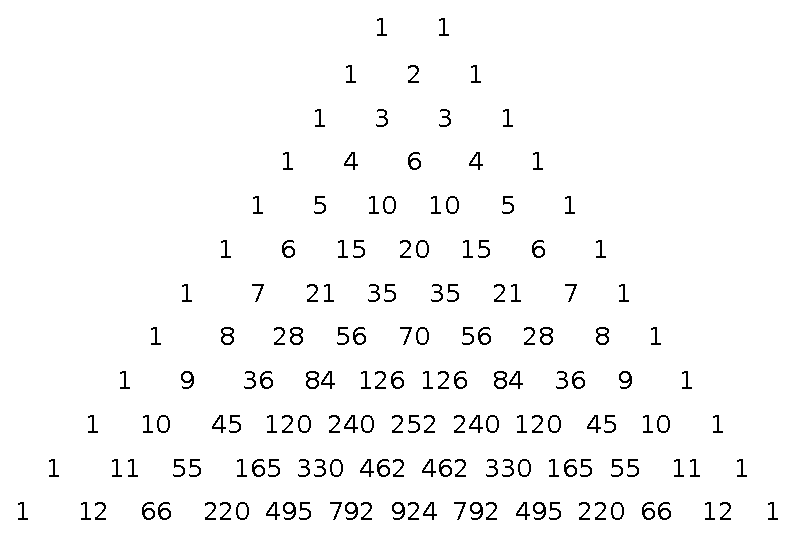
\includegraphics[scale=.8]{figure/fig1.eps}
\caption{}\label{fig01}
\end{figure}

rows from the top we have to book at row number $\alpha$ and row number $n-\alpha$ only, consider suitable products and take their maximum.

For $n=6$, $d=3$ we obtain $\tau = 10$, $\tau = 12$, $\tau_{3} = 9$ and $\tau = 12$. In the other hand $???$ can go upti $^6C_{3} = 20$ giving us several genuinely entangled vectors. It is clear how to proceed in general cases.
\end{example}
\end{proof}

Above results and discussion give complete information in certain special cases with a little more effort. We record them in the Example below.

\begin{example}\label{example-2.2}
 Let $F$, $\xi$ etc. be as above. Indeed we follow the notation terminology and results above freely. 
 
 \begin{enumerate}[label=(\roman*)]
 \item $\xi$ is a product vector in the following two cases
 
   \begin{enumerate}[label=(\alph*)]
   \item $l=1$, i.e; $F(\bold{\x}) = \lambda\bold{\x}^{k}$ for some scalar $\lambda \neq 0$ and $k \subset \Gamma_{n}$.
	\item $m=1$ i.e; $F(\bold{\x}) = a + b\x_{j}$ for some $j$ with $1 \leq j \leq n$ and $(a , b) \in \vertchar[.08ex]{C}^{2}$ with $b \neq 0$.
   \end{enumerate}
   
 \item Let us consider $F$ with $t \geq 2$, $m \geq 2$ and $d =1$. We have the following.
 
 \begin{enumerate}[label=(\alph*)]
 \item $\xi$ is not a product vector because $d < m$. Indeed, $F(\bold{\x}_{S_{F}})$ is irreducible. Here we set $F(\bold{\x}_{S_{F}}) = F(\bold{\x})$ only.
 \item If $S_{F} = \Gamma_{n}$, i.e; $m=n$, then $??$ is genuinely entangled. This does happen when $n=2$.
 \item Consider the case when $n \neq 3$ and $S_{F} \neq \Gamma_{n}$ and any ????? cut $(E, E')$. Then $???$ is a product vector in this cut if and only if either $E \supset S_{F}$ or $E' \supset S_{F}$.
  \end{enumerate}
 
 \item We now consider the case $n=2 =d = m \leq t$. Then $F$ has the form $F(\bold{\x}) = a_{0} + a_{1} \x_{1} + a_{2} \x_{2} + a_{3}\x_{1} \x_{2}$ with $a_{3} \neq 0$, $(a_{0}, a_{1}, a_{2}) \neq (0,0,0)$.
 
 \begin{enumerate}[label=(\alph*)]
  \item If $t=3$, then $\xi$ is entangled (and therefore, genuinely entangled).
 \item If $t = 2$ then the situation gets divided in three forms for $F$, viz, $F(\bold{\x}) = a_{0} + a_{3}\x_{1} \x_{2}$ with $a_{0} \neq 0$, giving rise to an entangled $\xi$ and $F(\bold{\x}) = a_{1}\x_{1} + a_{3}\x_{1}\x_{2} = \x_{1}(a_{1} + a_{3}\x_{2})$ with $a_{1}\neq  0$ or $F(\bold{\x}) = a_{2} \x_{2} + a_{3}\x_{1}\x_{2} = (a_{2} + a_{3}\x_{1})\x_{2}$ with $a_{2}\neq 0$. both giving rise to product vectors.
 
 \item If $t =4$, then each one of $a_{0}, a_{1}, a_{2}, a_{3}$ is non-zero. $\xi$ is a product vector if and only if $a_{0}a_{3}= a_{1}a_{2}$.
   \end{enumerate}
 
 \item Let $t=2$. Then $F(\bold{\x}) = a \bold{\x}^{k} + b \bold{\x}^{L}$ for some non-zero scalars $a$ and $b$ and distinct subsets $K$ and $L$ of $\Gamma_{n}$. So $F(\bold{\x}) = \bold{\x}^{K \cap L} (a \bold{\x}^{K L} + b \bold{\x}^{L K})$ and $K \triangle L = (K  L) \cup  (L K) \neq \phi$. We write $q(\bold{\x}_{K \triangle L})$ for the second factor. Then $q$ is irreducible.
 
 \begin{enumerate}[label=(\alph*)]
 \item $\xi$ is a product vector if and only if $\# K \triangle = 1$, i.e; either $K \subset L$ or $L \subset K$ and correspondingly $\#(L K) = 1$ or $\# (K L) = 1$.
 \item Given a bipartite cut $(E,E')$, $???$ is a product vector in this cut if and only if either $K \triangle L \subset E'$. This can happen only if $K \triangle ???$
 \item $\xi$ is genuinely entangled if and only if $K \cap L = \phi$ and $K \cup L = \Gamma_{n}$ i.e; $K \triangle L = \Gamma_{n}$ if and only if for $1 \leq j \leq n$, neither $\x_{j}$ is a factor of $F(\bold{\x})$ nor it is missing in $F(\bold{\x})$. 
 \end{enumerate}
 
 \item Let $t$ be any add prime.
 
 \begin{enumerate}[label=(\alph*)]
 \item $\xi$ is entangled because $t$ is not of the form $2^{u}$ for any non-negative integer $u$.
 \item $F(\bold{\x}) = \sum_{j=1}^{F} a_{j}\bold{\x}^{K_{j}}$ for some non-zero scalars $a_{j}$'s and distinct subsets $K_{j}$ of $\Gamma_{n}$. Let $K =\bigcap\limits_{j=1}^{t} K_{j}$, $L_{j} = K_{j} . ????$ for $1 \leq j \leq t$, $L =\bigcup\limits_{j=1}^{t}L_{j}$. Then $S_{F} = K \cup L = \bigcup\limits_{j=1}^{t} K _{j}$. Further $F(\bold{\x}) = \bold{\x}^{K}(\sum_{j=1}^{t} a_{j}\bold{\x}^{L_{j}})$. We write $q(\bold{\x}_{L})$ for the second factor. Then $q$ is irreducible because $t$ is prime and no $\x_{j}$ is a factor of $q(\bold{\x}_{L})$. Moreover, $S_{q} = L$ and $\# L \geq 2$.
 \item Give a biportite  and $(E, E')$, ??? product vector in this cut if and only ??? either $L \subset E$ or $L \subset E'$. This can happen only if $L ????$.
 \item $\xi$ is ???? entangled if and only if $K = \phi$ and $L = \Gamma_{n}$, i.e; $\bigcap\limits_{j=1}^{t} K, = \phi$ and $\bigcup\limits_{j=1}^{t} K = \Gamma_{n}$ of and nor $\x_{j}$ is missing in $F(\bold{\x})$.
  \end{enumerate}
 
 \end{enumerate}
 This ????? study to cases that ??? $n > 3$, $m \geq 2$, $d \geq 2$ and $???$ a composite number.
\end{example} 

\section{Polynomial Representation of Resonance Valence Bond States (RVB) and Their Quantum Entangement}\label{section-3}

For the sake of self-complateness and convenient notation and terminology we begin with the simple case of a singled a dimer and go upto that of ??? resonance ??? bond states with variable co-efficients. With the right choice made in Section~\ref{section-2} above, their polynomial representation turns ??? to be a homogeneous polynomial of small degree. This ??? the study of their quantum entanglement which requies new conditions that we introduce. For ???? we may refer to [1 to  12] or any other standard source.

\subsection{Basic definition and ????}\label{subsection-3.1}

Let $V \in \mathbb{N}$ and $n=2V$. We divide $\Gamma_{n} = \left\{j \in N : 1 \leq j \leq n\right\}$ into two equal parts $A$ and $B$, say $A = \left\{2^{t-1} : l \leq t \leq V\right\}$ and $B = \left\{ 2t : 1 \leq t \leq V \right\}$. For ?????? representations of various concepts we will mark points of $A$ by $\bullet$ and those of $B$ by $\odot$ and arrange them in different ways. For instance,

\begin{figure}
\centering
\includegraphics[scale=.8]{figure/fig2.eps}
\caption{}\label{fig02}
\end{figure}

is useful in the nearest neighbour (NN) context.

\begin{subsubsec}\label{subsubsection-3.1.1}
Coverings A bijective map $\Psi$ of $A$ to $B$ is called a covering, say $C$, of $\Gamma_{n}$. It can be given in terms of a permutation $\widetilde{\Psi}$ of $\Gamma_{n}$ by setting $\Psi(2t-1) = 2\widetilde{\Psi}(t)$ for $t \in \Gamma_{v}$.
  \begin{enumerate}[label=(\alph*)]
  \item $\Psi$ is called a nearest neighbour covering (???) $(NN)$ if $2(t-1) \leq \Psi(2t-1) \leq 2(t+1)$, i.e; $t-1 \leq \widetilde{\Psi}(t) \leq t H$(???) for $t \in \Gamma_{v}$. In other words, the permutation matrix of $\widetilde{\Psi}$ is handed matrix with band-width $\leq 1$.
   \item Samson and Ezermann [SE] study banded matrices and note in Remark 2.3 [SE] that the number of such matrices with bandwidth $\leq 1$ is the Fibonacci number $F_{v}$ with initial conditions $F_{1}=1 =F_{0}$.
   \item $\Psi$ is called a periodic $NN$ covering of we permit $\Psi(2v-1)$ to be 2 and $\Psi(1)$ to be 2v as well. In other words, we work in $\mathbb{Z} \md 2v$ .
   \item The number of all covering of $\Gamma_{n}$ is $\d{v}|$, the number of permutations of $\Gamma_{v}$.
    \item We will be considering various set $\underline{\overline\Psi}$ of covering with $\#\underline{\overline\Psi} \geq 2$ and $v \geq 2$. For $v=2$, $\#\underline{\overline\Psi}$ can only be 2, since the covering are only.
    
    \newpage
    
    \item Here are pictures of some easy coverings.
    
    \begin{figure}[h]
\centering
\includegraphics[scale=.8]{figure/fig3.1.eps}
\caption{}\label{fig03}
\end{figure}

  \end{enumerate}
\end{subsubsec}

%%%%%%%%%%%%%%%%%%%%%%%%%%%%%%%%21 page %%%%%%%%%%%%%%%%%%%%%%%%%%%%%%%%%%%%%%%%%%%%%%%%%%%%%%%%%%%%%%%%%%%%%
\begin{subsubsec}\label{subsubsection-3.1.2}

{\bfseries Resonance valence bond (RVB) states and Vectors.}

For $a\in A$, $b \in B$, we write $H_{a,b}$ for $\mathcal{H}_{a} \bigotimes \mathcal{H}_{b}$. We follow the polynomial representation as set out in section~\ref{section-2} above.

\begin{enumerate}[label=(\alph*)]
\item A dimer or a singlet at a, b is the unit vector
$$
[a, b] = \frac{1}{\sqrt{2}} (| \uparrow \rangle_{a} \otimes | \downarrow \rangle_{b}) = \frac{1}{\sqrt{2}}(| 0\rangle_{a} \otimes | \shortmid \rangle - | \shortmid \rangle_{a} \otimes | 0 \rangle_{b})\quad {\rm in} \quad  \mathcal{H}_{a,b} 
$$

Its polynomial representation is given by
\begin{equation*}
F_{a_{1}b}(\x_{a}, \x_{b}) = \frac{1}{\sqrt{2}}(\x_{b}- \x_{a})\tag{3.3}
\end{equation*}

\item Let  $C$ be a covering of $\Gamma_{n}$ i.e; a bijective map $\Psi$ of $A$ to $B$. We let $| C \rangle = | \Psi \rangle$ be the vector in $\mathcal{H}$ identified with $\bigotimes\limits_{a \in A} \quad \mathcal{H}_{a}\Psi_{(a)}$ given by $\bigotimes\limits_{a \in A} [a, \Psi(a)]$, i.e;,
\begin{gather*}
2^{-v/2} \bigotimes\limits_{a \in A} \left(| \uparrow \rangle_{a} \otimes | \downarrow \rangle_{\Psi (a)}) - | \downarrow \rangle_{a} \otimes | \uparrow \rangle_{\Psi (a)}\right)\\
= 2^{-v/2} \bigotimes\limits_{a\in A} \left(|0\rangle_{a} \otimes | 1 \rangle_{\Psi(a)} - |1 \rangle_{a} \otimes | 0 \rangle_{\Psi(a)}\right)
\end{gather*}
 
 
It is a unit vector and its polynomial representation is 
\begin{equation}
F_{\underline{\overline{\Psi}}} = 2^{-v/2} \prod\limits_{a\in A}(\x_{\Psi(a)}- \x_{a})\tag{3.4}\label{eq-3.4}
\end{equation}

It is a non-zero homogeneous polynomial of degree $d=v$ and its support is $S_{F_{\underline{\overline{\Psi}}}} = \Gamma_{n}$, i.e., $m=n$.

Indeed, 
\begin{align*}
F_{\Psi}(\bold{\x}) &= 2^{-v/2} \sum_{A_{1} \subset A}(-1)^{??? A_{1}} \bold{\x}^{A_{1}} \bold{\x}^{B\smallsetminus\Psi(A_{1})}\nonumber\\
& = 2^{-v/2} \sum_{\substack{A_{1} \subset A \\ \#A_{1} \leq v/2 \\ | \in A_{1}={\rm nu}/2 }} \left(\bold{\x}^{A_{1}} \bold{\x}^{B\smallsetminus \Psi (A_{1}) } + (-1)^{v} \bold{\x}^{A \smallsetminus A_{1}} \bold{\x}^{\Psi (A_{1})} \right)\tag{3.5}  
\end{align*}

Clearly, the number $t$ of terms in $F_{\Psi}$ is $2^{v}$ and $\bold{\x}^{k}$ is not a factor of $F_{\Psi}(\bold{\x})$ for any $\phi \neq K_{\neq} \subset \Gamma_{n}$.

\item Let $v \geq 2$ and $\underline{\overline{\Psi}}$ a set of coverings of $\Gamma_{n}$ with $s= \# \underline{\overline{\Psi}} \geq 2$. Then we write $| \underline{\overline{\Psi}}\rangle$ for the RVB vector $\frac{1}{\# \underline{\overline{\Psi}}} \sum_{\Psi \in \underline{\overline{\Psi}}} | \Psi \rangle$ in $\mathcal{H}$. We note that $|| \underline{\overline{\Psi}} || \leq |$ and we will come to its normalization later in (3.1.4).

\item The polynomial representation of $| \underline{\overline{\Psi}}\rangle$ is given by
\begin{equation}
F_{\underline{\overline{\Psi}}} = \frac{1}{\# \underline{\overline{\Psi}}} \sum_{\Psi \in \underline{\overline{\Psi}}} F_{\Psi} = \frac{1}{\# \underline{\overline{\Psi}}} \sum_{\substack{{A_{1} \subset A}\\ B_{1}\subset, \# B_{1}= \# A_{1}}} (-1)^{\# A_{1}} \# \left\{ \Psi \in \underline{\overline{\Psi}} : \Psi (A_{1}) = B_{1}\right\} \bold{\x}^{A_{1}} \bold{\x}^{B\smallsetminus B_{1}}\tag{3.6}\label{eq-3.6}
\end{equation}

Then $| \underline{\overline{\psi}} \rangle \neq 0$ simply because $0 \neq 2^{-v/2}(\bold{\x}^{B} + (-1)^{v} \bold{\x}^{A})$ is a part of $F_{\underline{\overline{\Psi}}}(\bold{\x})$.

Indeed, this also gives that $S_{F_{\underline{\overline{\Psi}}}} = \Gamma_{n}$, i.e., $m=n$ and $\bold{\x}^{K}$ is not a factor of $F_{\underline{\overline{\Psi}}} (\bold{\x})$ for any $\phi \neq K \subset \Gamma_{n}$.

\item Let $v \geq 2 $, $\underline{\overline{\Psi}}_{NN} =$ the set of nearest neighbour $(NN)$ coverings of $\Gamma_{n}$ and $\underline{\overline{\Psi}}_{PNN} =$ the set of periodic nearest neighbour $(PNN)$  covering of $\Gamma_{n}$. Then $|\underline{\overline{\Psi}}_{NN} \rangle$ and $| \underline{\overline{\Psi}}_{PNN} \rangle$ will be called the NN-RVB and the PNN-RVB vectors (in the context of n-qubit system).

We record some immediate applications of Theorem~\ref{thm-2.1}, 2.2 above is section~\ref{section-2} labelled as Theorem~\ref{thm-3.1} and Example~\ref{example-3.1}.

\end{enumerate}

\end{subsubsec}

\begin{thm}\label{thm-3.1}

We consider the vectors given in~\eqref{subsubsection-3.1.2} above in their respective spaces.

\begin{enumerate}[label=(\roman*)]

\item A dimer $[a, b]$, $| \Psi \rangle$, $| \underline{\overline{\Psi}} \rangle$ are all entangled.

\item Let $v \geq 2$ and $(E, E')$ a  bipartite cut of $\Gamma_{n}$.

   \begin{enumerate}[label=(\alph*)]
    \item $| \Psi \rangle$ is a product vector in the cut $(E, E')$ if and only if 
			\begin{align*}
			\Psi(E \cap A) &= E \cap B \quad \text{if and only if}\\
			\Psi(E' \cap A) &= E'\cap B \tag{3.7}\label{eq-3.7}
			\end{align*}
			
	 In this case we have $\# E$ and $\# E'$ are both even.
	 \item If $| \underline{\overline{\Psi}} \rangle$ is a product vector in the cut $(E, E')$, then 
	 		\begin{equation}
	 		 \Psi(E \cap A) = E \cap B \quad ({\text {equivalently}}, \Psi (E' \cap A) = E' \cap B)\; \text{for each}\; \Psi \;\text{in}\; \underline{\overline{\Psi}}\tag{3.8}\label{eq-3.8}   
	 		\end{equation}
	 		
	 	In this case, $\# E$ and $\# E'$ are both even.	
    \end{enumerate}
    
   \item For $v=2$, $| \underline{\overline{\Psi}} \rangle$ is genuinely entangled.
   
   \item For $\underline{\overline{\Psi}} $ NN or PNN, $|\underline{\overline{\Psi}}\rangle$ is genuinely entangled.
   
   \item (a) The converse of (ii) (b) holds for $v=3$ but not in general.
   
   (b) The converse of (ii) (b) holds for all $v \geq 3$ if we consider special cuts with $\min \left\{ \# E, \# E' \right\} = 2$.
\end{enumerate}
\end{thm}

\begin{proof}
\begin{enumerate}[label=(\roman*)]
 
 \item  It follows from Theorem~\ref{thm-2.1} (i) (a) because $d=v < 2 v =n$ for the corresponding polynomials. 

\item (a) The second equivalence is trivial. For the first one, the `if' part is immediate. For the  `only if' part, let, $p(\bold{\x}_{E}), q (\bold{\x}_{E'})$ be polynomials that satisfy $F(\bold{\x}) = p(\bold{\x}_{E}) q(\bold{\x}_{E'})$. Then by Theorem~\ref{thm-2.1} (iv) (b), $p(\bold{\x}_{E})$ and $q(\bold{\x}_{E'})$ are both homogeneous, say, of degree $v_{1}$ and $v_{2}$ respectively with $v_{1} \geq 1$, $v_{2} \geq 1$, $v_{1} + v_{2} = v$, $S_{p} =E$ and $S_{q} = E'$.  low by~\eqref{subsubsection-3.1.2} (b) $\bold{\x}^{A}$ and $\bold{\x}^{B}$ both occur in $F_{\Psi}(\bold{\x})$. The one and only one way it can happen is the $\bold{\x}^{E \cap A}$, $\bold{\x}^{E \cap B}$ occur in $p(\bold{\x}_{E})$, and $\bold{\x}^{E' \cap A}$ and $\bold{\x}^{E' \cap B}$ occur in $q(\bold{\x}_{E'})$. This gives that $\# E \cap A = \# E \cap B = v_{1}$ and $\# E' \cap A = \# E' \cap B =v_{2}$. Now $\bold{\x}^{E \cap A}$ $\bold{\x}^{E' \cap B}$ occurs in But this can happen for $F_{\Psi} (\bold{\x})$ if and only of $B \Psi(E \cap A) = E' \cap B$, i.e., $\Psi(E \cap A) = E \cap B$. As a consequence $\Psi (E' \cap A) = E' \cap B$ as well. This confirms the assertion already made about the relationships amongst cardinalties of the sets, $v_{1}$, $v_{2}$. Clearly $\# E = \# (E \cap A) + \# (E \cap B) = 2 v_{1}$.

(b) As noted in ~\ref{subsubsection-3.1.2} (c), $\bold{\x}^{A}$ and $\bold{\x}^{B}$ both occur in $F_{\overline{\Psi}}(\bold{\x})$. So arguments in the proof of part (ii) (a) above by replacing $F_{\Psi}$ by $F_{\underline{\overline{\Psi}}}$ with the addition of ``for some $\Psi \in \underline{\overline{\Psi}}$ in the sentence beginning with `But'. Now consider any $\varphi \in \underline{\overline{\x}}$. Then $\bold{\x}^{E \cap A} \bold{\x}^{B \smallsetminus \varphi (E \cap A)}$ occurs in $F_{\underline{\overline{\Psi}}}(\bold{\x})$ and, therefore, in $p(\bold{\x}_{E}) q(\bold{\x}_{E'})$. The only way this can happen is that $B \smallsetminus \varphi (E \cap A) = E' \cap B$, which gives, in turn, $\varphi(E \cap A) - E \cap B$. This completes the proof of the first assertion. The second statement following ?????.

\item For $v=2$, the condition~\ref{eq-3.8}   in (ii) (b) is note satisfied for any $\phi \neq E \subset \lceil_{4}$ as in clear from ~\ref{subsubsection-3.1.2} (e) above. (iii) It follow $\langle \neq \#$ from (ii)(b) and (c).

\item In view of (iii), it is enough to consider the case $v \geq 3$. Let, if possible, the condition in (ii) (b) the case $v \geq 3$. Let if possible, the condition in (ii)(b) be satisfied for some $E$ with $\phi \neq E_{\neq} \subset \neq_{n}$ and $\underline{\overline{\Psi}}= \underline{\overline{\Psi}}_{NN}$.

Consider any $2s-1 \in E \cap A$ with $1 \leq s\ leq v$. If $s < v$, then there exist $\Psi_{1}, \Psi_{2} \in \underline{\overline{\Psi}}$ with $\Psi_{1} (2s-1) = 2(s + 1)$ and $\Phi_{2} (2s+1) = 2(s+ 1)$. So $s(s+ 1) \in E \cap B$, which in turn, gives that $2s+1 \in E \cap A$. On the other hand, if $s > 1$, then there exist $\Psi_{3}, \Psi_{4} \in \underline{\overline{\Psi}}$ satisfying $\Psi_{3}(2s-1)= 2(s-1)$ and $\Psi_{3}(2s-3) =2 (s-1)$. So $2(s-1) \in E \cap B$ which leads to $2s-3 \in E \cap A$. Repeating the arguments iteratively we arrive at the conclusion that $\left\{2t-1 : 1 \leq t \leq v \right\} \subset E \cap A$. But that is not so. Hence $\underline{\overline{\Psi}}_{NN}$ is note a product vector in any bi?????? cut and is therefore genuinely entangled.  

Now we come to $\underline{\overline{\Psi}}_{PNN}$. Because $\underline{\overline{\Psi}}_{PNN} \supset \underline{\overline{\Psi}}_{NN}$, it cannot satisfy (\ref{subsection-3.6}) in (ii)(b) for any $E$ with $\phi \neq E \subset_{\neq} \Gamma_{n}$. Hence $\underline{\overline{\Psi}}_{PNN}$ is genuinely entangled.

\item 
\begin{enumerate}[label=(\alph*)]
\item For any bipartite cut $(E, E')$ of $\lceil_{6}$ with $\#E$ and $\#E'$ both even,\break $\min\left\{\# E, \# E'\right\}=2$. Suppose $\#E'=2$. Then for any $\Psi \in \underline{\overline{\Psi}}$, $\Psi (E' \cap A) = E' \cap B$,say, $\Psi(a) = b$ where $E'\cap A = \{a\}$, $E'\cap B=\{b\}$. So $\x_{b} \smallsetminus \x_{a}$ is a factor of $F(\bold{\x})$. Similarly for the case of $\# E=2$. So $\lceil\underline{\Psi}\rangle$ is a product vector in the cut $(E, E')$ by Theorem~\ref{thm-2.1}(ii)(a).

We shall give an example in Example~\ref{example-3.1} below to show that the converse of (ii)(b) in Theorem here does not hold in general.

\item We can formulate the proof on the lines of that of (a) above.

\end{enumerate}

\end{enumerate}

\end{proof}


\begin{definition}\label{def-3.1}
(i) We call $\underline{\overline{\Psi}}$ $\boldsymbol{\text{decomposable Via} ~E}$ if it satisfies the condition~\ref{subsection-3.6} in Theorem~\ref{thm-3.1}(ii)(b) above, i.e; $\Psi(E\cap A) = E\cap B$ for $\Psi \in \underline{\overline{\Psi}}$. (ii) $\underline{\overline{\Psi}}$ will be called $\boldsymbol{\rm decomposable}$ if it is decomposable via $E$ for some bipartite cut $(E, E')$. 
\end{definition}

\begin{example}\label{example-3.1}
We consider~\ref{subsubsection-3.1.1} $(F)$ above and use Theorem~\ref{thm-3.1} above freely.
\end{example}

\begin{enumerate}
\item Let $v=3$ and $\underline{\overline{\Psi}}$ consist of the two converings given in Figures. Then $\underline{\overline{\Psi}}$ is not decomposable. So $\lceil\underline{\Psi}$ is genuinely entangled.

\item Let $v=4$ and $\underline{\overline{\Psi}}$ consist of the two coverings in Figure\ref{fig03}. Then $\underline{\overline{\Psi}}$ is decomposable with $E= \{3,4,5,6\}$ serving the desired purpose. However,$\lceil\underline{\overline{\cup}}\rangle$ is note a product vector in the bipartite cut $(E, E')$  as can be seen by computing $F_{\underline{\overline{\Psi}}}$. In fact,
\begin{equation*}
\begin{split}
F_{\underline{\overline{\Psi}}}(\bold{\x}) = &\left(\x_{2} \x_{8} + \x_{1}\x_{7} - \x_{1}\x_{2} -\x_{7}\x_{8}\right)\left(\x_{4}\x_{6} + \x_{3}\x_{5}- \x_{3}\x_{4} - \x_{5}\x_{6} \right)\\
&+ \left(\x_{2}\x_{8} + \x_{1}\x_{7} - \x_{1}\x_{8}-\x_{2}\x_{7}\right) \left(\x_{4} \x_{6} + \x_{3} \x_{5} - \x_{3}\x_{6}-\x_{4} \x_{5}\right).
\end{split}
\end{equation*}

This can note be factored as as $p(\bold{\x}_{E})~q(\bold{\x}_{E'})$ for any polynomials $p$ and $q$ more are apart from $E$ there is no other subset $G$ with $\phi \neq G \subset_{\neq} \lceil_{6}$ that satisfies the condition~\ref{subsection-3.6} of decomposability. This show that the converse of Theorem~\ref{thm-3.1}(ii)(b) does not hold in  general.
\end{enumerate}

\begin{subsubsec}\label{subsubsection-3.1.3}
${{\text{\bf Concepts and properties if}}~ \mathbf{\underline{\overline{\Psi}}}~ \text{\bf related to decomposability}}.$

Let $v\geq 3$ and $\# \underline{\overline{\Psi}} \geq 2$.

\begin{enumerate}[label=(\alph*)]

\item  Let $\varphi_{1} = \left\{A_{1} \subset A : \# \left\{\Psi (A_{1}) : \Psi \in \underline{\overline{\Psi}} \right\} \right\} =1$. For $A_{1} \in \varphi_{1}$ we write $B_{1}$ for $\Psi(A_{1})$ for any (and thus for all) $\Psi \in \underline{\overline{\Psi}}$. Then $\phi, A \in \varphi_{1}$ and $\varphi_{1}$ is an algebra of subsets of $A$. As a consequence, $B_{1} = \left\{B_{1}= \Psi(A_{1}) : A_{1} \in \varphi_{1} \right\}$ is an algebra of subsets of $B$. In particular, \# $\varphi_{1} \geq 3$ if and only if \# $B_{1} \geq 3$. In this case, let $\varphi_{1}$ mix be the subset of $\varphi_{1}\{\phi\}$ consisting of its minimal subsets.

\item Now suppose \# $\varphi_{1} \geq 3$ and consider any $A_{1} \in \varphi_{1}$ with $\phi \neq A_{1}\neq A$. We set $E = A_{1} \cup B_{1}$. Then \# $E \neq \Gamma_{n}$. Also $\Psi(E \cap A) = E \cap B$ for $\Psi \in \underline{\overline{\Psi}}$. In other words, $\underline{\overline{\Psi}}$ is decomposable via $E$. for $\Psi \in \underline{\overline{\Psi}}$. In other words, $\underline{\overline{\Psi}}$ is decomposable via $E$. Then $\phi \neq E \cap A \neq A$ and $E \cap A \in \varphi_{1}$. This in then, gives that \# $\varphi_{1} \geq 3$. 

\item Because \# $\underline{\overline{\Psi}} \geq 2$, there exist $\Psi_{1}, \Psi_{2} \in \underline{\overline{\Psi}}$, $a \in A$, $b_{1} \neq b_{2}$ in $B$ with $\Psi_{1}(a_{1}) = b_{1}$, $\Psi_{2}(a_{1}) = b_{2}$. So $\{a_{1}\} \in \varphi_{1}$. Hence $\varphi_{1} \neq P_{A}$. Can de??? $\varphi_{1}$ is an algebra of subsets of $A$ too.

\item Consider $a_{1}$ as in (c) above and $a_{2}\neq a_{1}$ in $A$. If $\left\{a_{1}, a_{2} \right\} \in \varphi_{1}$ then $\Psi_{1}\left\{a_{1}, a_{2} \right\} = \left\{b_{1},\Psi_{1} (a_{2})\right\}$ has to be $\Psi_{2}\left\{a_{1}, a_{2} \right\} = \left\{b_{2},\Psi_{2} (a_{2})\right\}$ so that $\Psi_{1}(a_{2}) = b_{2}$ and $\Psi_{2}(a_{2}) = b_{1}$ and, thus, $\left\{a_{2}\right\} \notin \varphi_{1}$. On the other hand, if $\left\{a_{2}\right\} \in \varphi_{1}$, then $\Psi_{1}\left\{a_{1}, a_{2}\right\} = \left\{b_{1}, \Psi_{1}(a_{2})\right\} = \left\{b_{1}, \Psi_{2}(a_{2})\right\} \neq \left\{b_{2}m \Psi_{2}(a_{2})\right\}$ and, thus $\left\{a_{1}, a_{2} \notin \varphi_{1}\right\}$. Hence\, at most one of $\left\{a_{2}\right\}$, $\left\{a_{1}, a_{2}\right\}$ is in $\varphi_{1}$.

\item Let $\varphi_{2} = \left\{A_{2} \subset A : \# \{\Psi (A_{2}) : \Psi \in \underline{\overline{\Psi}}\} \geq 2\right\}$. Then $\varphi_{1} \cap \varphi_{2} = \phi$, $\varphi_{1} \cup \varphi_{2} = P_{A}$ and for $A_{2} \in \varphi_{2}$, $A \smallsetminus A_{2} \in \varphi_{2}$. By (c) above $\{a_{1}\} \in \varphi_{2}$ and therefore, $A\smallsetminus \{a_{1}\}$ and $\{a_{1}, a_{2}\}$ Now by (d), for $a_{2}\in A\smallsetminus\{a_{1}\}$, at least one of $\{a_{2}\}$
and $\{a_{1}, a_{2}\}$ is in $\varphi_{2}$ and neither of them or their complements in $A$ equal $\{a_{1}\}$ or $A\smallsetminus\{a_{1}\}$ because $v\geq 3$. Hence $\# \varphi_{2}\geq 4$.

\item $\phi$ and $A$ are in $\varphi_{1}$ and therefore, not in $\varphi_{2}$. So for $A_{2} \in \varphi_{2}$ $v-1 \geq \#$ $A_{2}\geq 1$ and, therefore, $^{v}C_{\# A_{2}} \geq v$.

\item 
\begin{align*}
F_{\underline{\overline{\Psi}}}(\bold{\x}) &= 2^{-v/2} \sum_{A_{1} \in \varphi_{1}}(-1)  \bold{\x}^{A_{1}} \x^{B\smallsetminus B_{1}} + \\
   & 2^{-v/2} \frac{1}{\# \underline{\overline{\Psi}}} \sum_{A_{2} \in \varphi_{2}} (-1)^{\# A_{2}} ??? \left(\sum_{B_{2} \in B} \# \left\{\Psi \in \underline{\overline{\Psi}} : \Psi(A_{2}) - B_{2}\right\}\bold{\x}^{B\smallsetminus B_{2}}\right)\tag{3.9}
\end{align*}

\item Let $A_{2} \in \varphi_{2}$. We write, for $B_{2} \subset B$, $A_{2}, B_{2}$ for $\frac{1}{\#\underline{\overline{\Psi}}} \# \{\Psi \in \underline{\overline{\Psi}} : \Psi (A_{2}) = B_{2} \}$. which in $\geq 0$.

We note that $C_{A_{2}B_{2}} \neq 0$ if and only if $B_{2} \in \{ \Psi (A_{2}) : \Psi \in \underline{\overline{\Psi}}\}$ .

In Particular, $C_{A_{2}B_{2}} = 0$ for $\# A_{2} \neq \# B_{2}$. Moreover $\sum_{B_{2 \subset B}}$ $C_{A_{2}, B_{2}} =1$ so $^{v}C_{\# A_{2}} \geq \# \{B_{2} \subset B : C_{A_{2}, B_{2}} \neq 0 \} \geq 2$.

This, in turn, gives that $C_{A_{2}, B_{2}}>0$ for at last two distinct subsets $B_{2}$ of $B$. As a consequence, $C_{A_{2}, B_{2}} < 1$ for all $B_{2} \subset B$.

\item Let 
\begin{align*}
F^{1}_{\underline{\overline{\Psi}}}(\bold{\x})  &= 2^{-v/2} \sum_{A_{1} \in \varphi_{1}}(1)^{\# A_{1}} \bold{\x}^{A_{1}} \bold{\x}^{B\smallsetminus} B_{1}\\
F^{2}_{\underline{\overline{\Psi}}}(\bold{\x})  &= 2^{-v/2} \sum_{A_{2} \in \varphi_{2}} \sum_{B_{1} \subset B} C_{A_{2}, B_{2}}(-1)^{\# A_{2}} \bold{\x}^{A_{2}} \bold{\x}^{B\smallsetminus}B_{2}\tag{3.10}\\
\text{So}\quad\quad F_{\underline{\overline{\Psi}}} (\bold{\x}) &= F^{1}_{\underline{\overline{\Psi}}} (\bold{\x}) + F^{2}_{\underline{\overline{\Psi}}} (\bold{\x})
\end{align*}

Let $t$, $t^{(1)}$, $t^{(2)}$ be the number of terms in $F_{\underline{\overline{\Psi}}}(\underline{x})$, $F^{(1)}_{\underline{\overline{\Psi}}}(\underline{x})$ and $F^{(2)}_{\underline{\overline{\Psi}}}(\underline{x})$ respectively then $t^{(1)} = \# \varphi_{1}$.

Using (h), we have $\sum_{A_{2} \in \varphi_{2}} \quad ^{v}C_{\# A_{2}} \geq t^{(2)} \geq 2 \# \varphi_{2}$. But by (e), $\# \varphi_{2} \geq 4$  and therefore, $f^{(2)} \geq 8$. Hence 
\begin{align*}
2^ {v} + \sum_{A_{2} \in \varphi_{2}}(^{v}C_{\# A_{2}}-1) &= \# \varphi_{1} + \sum_{A_{2} \in \varphi_{2}} ^{v}C_{\# A_{2}} \geq t^{(1)} + t^{(2)} = t \geq \# \varphi_{1} + 2 \# \varphi_{2} = \#P_{A} + \# \varphi_{2}\\
& = 2^{v} + \# \varphi_{2} \geq 2^{v} + 4 \tag{3.11}  
\end{align*}

\item If $\{a\} \in \varphi_{1}$ for some $a\in A$, then by (b) above and Theorem~\ref{thm-3.1} (v)(b), $|\underline{\overline{\Psi} \rangle}$ is a product vector in the bipartite cut $(E, E')$ with $E= \{a\}$.

\item We confine out attention to the case that $\{a\} \notin \varphi_{1}$, $a\in A_{1}$. In that case, $\{a\} \in \varphi_{2}$ for $a\in A$. So $\# \varphi_{2} \geq 2v$ because $\{A \smallsetminus \{a\}, \{a\} : a \in A \}$ are all different sets in view $v \geq 3$. This refines the second part of (3.11) viz; 
\begin{equation*}
t \geq 2^{v} + \# \varphi_{2} \geq 2^{v} + 2 \Psi = 2(2^{v-1} + v)\tag{3.12} 
\end{equation*} 

\end{enumerate}

We record a few test of decomposability which are ????? in 3.1.3 (a)\& (b), (i) and (k) above.

\end{subsubsec}

\begin{thm}\label{3.2}
{\bf (Tests of decomposability)}. Let $v\geq 3$ and $\# \underline{\overline{\Psi}} 2$.
\begin{enumerate}[label=(\roman*)]
\item The following are equivalent
\begin{enumerate}[label=(\alph*)]
\item $\underline{\overline{\Psi}}$ is decomposable.

\item $\# \varphi_{1} \geq 3$

\item $\# \varphi_{1} \geq 4$

\item The number $s$ of terms in $F_{\underline{\overline{\Psi}}}(\bold{\x})$ with $|$co-efficient$|= 2^{-v/2}$ is $\geq 3$.

\item The number $s$  as in (d) above is $\geq 4$.

\end{enumerate}

\item If $t < 2^{v} + 2v$ then $\underline{\overline{\Psi}}$ is decomposable via  some $a \in A$. Further in this case $| \underline{\overline{\Psi}} \rangle$ is a product vector in the bipartite cut $(E, E')$.
\end{enumerate}

\end{thm}

\begin{subsubsec}\label{subsubsection-3.1.4}
{\bf Normarization of $| \underline{\overline{\Psi}} \rangle$}. Let $v \geq 2$ and $\# \underline{\overline{\Psi}} \geq 2 $. (a) By \ref{subsubsection-3.1.1} (e) for $v=2$, there is only one $\underline{\overline{\Psi}}$. 

The polynomial representation of $| \underline{\overline{\Psi}} \rangle$ is given by
\begin{align*}
F_{\underline{\overline{\Psi}}} (\bold{\x}) &= \frac{1}{z^{2}}\left((\x_{2} - \x_{1}) (\x_{4} - \x_{3}) + (\x_{4}-\x_{1}) (\x_{2}-\x_{3})\right)\\
 &= \frac{}1{4} \left(2(\x_{1} \x_{3} + \x_{2} \x_{4}) - \x_{1} \x_{4}- \x_{2}\x_{3} -\x_{1}\x_{2}-\x_{3}\x_{4}\right)\\
\text{So} \quad || | \underline{\overline{\Psi}} \rangle || &= \frac{1}{4} \sqrt{\left(4+4+1+1+1+1\right)} = \frac{\sqrt{3}}{2}\tag{3.13}
\end{align*}

Hence the corresponding RVB state is $| \underline{\overline{\Psi}} \rangle  = \frac{2\sqrt{3}}{3} | \underline{\overline{\Psi}} \rangle$ and its polynomial representation is given by 
\begin{equation*}
F_{\underline{\overline{\Psi}}}(\bold{\x}) = \frac{\sqrt{3}}{6} \left(2(\x_{1}\x_{3} + \x_{2}\x_{4}) - \x_{1}\x_{4} - \x_{2}\x_{3}- \x_{1}\x_{4} -\x_{3}\x_{4}\right)\tag{3.14}
\end{equation*}

Let $v\geq 3$. We use\ref{subsubsection-3.1.3}(i). The terms of the polynomial representation of $F_{\underline{\overline{\Psi}}}(\bold{\x})$ coming from non-zero values of $C_{A_{2}, B_{2}}$'s are mutually orthogonal in $\lfloor^{2}\left(\prod^{n}\right)$, So
\begin{equation*}
|| | \underline{\overline{\Psi}} \rangle || = ||F_{\underline{\overline{\Psi}}}(\bold{\x})||_{2} = 2^{-v/2}\sqrt{\left(\# \varphi_{1}  + \sum_{A_{2} \in \varphi_{2}} \left(\sum_{B_{2} \subset B} C_{A_{2}, B_{2}}^{2}\right) \right)}\tag{3.15}
\end{equation*}

But for each $A_{2} \in \varphi_{2}$, $\# \{B_{2} \subset B  : C_{A_{2}, B_{2}} \neq 0\} \geq 2$ and $\sum C_{A_{2}, B_{2}} = 1$; by \ref{subsubsection-3.1.3} (h). So $\sum_{B_{2} \in B} C_{A_{2}, B_{2}} < 1$ for $A_{2} \in \varphi_{2}$.

Hence
\begin{equation*}
|| | \underline{\overline{\Psi}} \rangle || < 2^{-v/2} (\# \varphi_{1} + \# \varphi_{2}) =1\tag{3.16}
\end{equation*}

The corresponding RVB state, say $\widetilde{| \underline{\overline{\Psi}} \rangle} = \frac{1}{|| | \underline{\overline{\Psi}} \rangle||} | \underline{\overline{\Psi}} \rangle$ and its polynomial representation is 
\begin{equation*}
\widetilde{F}_{\underline{\overline{\Psi}}} (\bold{\x}) = \frac{1}{|| | \underline{\overline{\Psi}} \rangle||} F_{\underline{\overline{\Psi}}}(\bold{\x})\tag{3.17}
\end{equation*}

\end{subsubsec}

\begin{subsubsec}\label{subsubsection-3.1.5}
{\bf Motivation for factor ability of sets of coverings}. Theorem~\ref{thm-3.1} and \ref{subsubsection-3.1.3} permit us to confine out attention to $v\geq 3$ and decomposable coverings $\underline{\overline{\Psi}}$ with $\# \underline{\overline{\Psi}} \geq 2$ and $\{a\} \notin \varphi_{1}$, for any $a \in A$ on the one hand and motivate the new concept of factorability of $\underline{\overline{\Psi}}$ on the other hand.

%%%%%%%%%%%%%%%%%%%%%%%%%%%%%%%%%31%%%%%%%%%%%%%%%%
\begin{enumerate}[label=(\alph*)]
\item Suppose $\underline{\overline{\Psi}}$ is decomposable via $E$. Let $v_{1}= \# E \cap A$, $v_{2} = \# E' \cap A$

Let $\overline{\bold{\Psi}}_{E} = \left\{ \Psi /E : \Psi \in \overline{\bold{\Psi}}\right\}$ and $\overline{\bold{\Psi}_{E'}} = \left\{\Psi/E^{-1}: \Psi \in \overline{\bold{\Psi}}\right\}$.

We may set up label things $\left\{\Psi_{\alpha}^{E} : 1 \leq j \leq j^{1} \right\}$ and $\left\{\Psi_{k}^{E'} : 1 \leq k \leq k'\right\}$ for $\overline{\bold{\Psi}}_{E}$ and $\overline{\bold{\Psi}}_{E'}$ respectively. Then $\max\left\{j^{-1}, k'\right\} \geq 2$ simply because $\# \overline{\bold{\Psi}} \geq 2$. 

\item For any bijective  maps $\Psi_{1} : E \cap A \longrightarrow E \cap B$ and $\Psi_{2} : E' \cap A \longrightarrow E' \cap B$

We write $\Psi_{1} \times \Psi_{2}$ for the bijective map of $A$ to $B$ given by
\[
(\Psi_{1} \times \Psi_{2})~(a) =  
\begin{cases*}
\Psi_{1}(a),~~ \text{if}~~ a\in E\tag{3.18} \\
\Psi_{1}(a),~~ \text{if}~~a \in E' 
\end{cases*}
\]

For instance, $\Psi \in \overline{\bold{\Psi}}$ can be written as $\Psi_{E} \times \Psi_{E'}$.

\item Let $\overline{\bold\Phi}_{1}$ and $\overline{\bold{\Phi}}_{2}$ be any two sets of bijective maps $\varphi_{1}$ and $\varphi_{2}$ of in $E \cap A$ to $E \cap B$ and on $E' \cap A \rightarrow E' \cap B$  respectively. These we denote $\{ \varphi_{1} \times \varphi_{2} : \varphi \in \overline{\bold\Phi}_{1}, \varphi_{2} \in \overline{\bold\Phi}_{2}\}$ by $\overline{\bold\Phi}_{1} \times \overline{\bold\Phi}_{2}$.

\item For the sake of conveniende, we call $\psi_{1}$ and $\psi_{2}$ as in (b) \textbf{converings of $\mathbf{E}$ and $\mathbf{E'}$} respectively. We note 
that

 \begin{equation}
 \overline{\bold{\psi}}=????_{\Psi \in \overline{\bold\Psi}} \left(\{\psi/E\} \times \{\psi/E' \} \right) \quad \overline{\bold\psi}_{E} \times \overline{\bold\psi}_{E'} = \left\{\psi_{j}^{E} \times \psi_{R}^{E'} : 1 \leq j \leq j', 1 \leq k \leq k'\right\}\tag{3.19}\label{eq-3.19}
 %~ \overline{\bold{\psi}} = ????_{\Psi \in \overline{\bold\Psi}}} \left(\{\psi/E\} \times \{\psi/E' \} \right)
 %~ \quad \overline{\bold\psi}_{E} \times \overline{\bold\psi}_{E'} = \left\{\psi_{j}^{E} \times \psi_{R}^{E'} : 1 \leq j \leq j', 1 \leq k \leq k'\right\}
\end{equation}


\item We may picuture $\overline{\bold\psi}_{E} \times \overline{\bold\psi}_{E'}$ as a rectangular array $\varphi$ of dots, or, for that matter the $k' \times j'$ matrix $M$ with all entries 1. The $\overline{\bold\Psi}$ is a subset of $R$. haring at least on dot in each row and at least one dot in each column. The corresponding matrix for $\overline{\boldsymbol{\psi}}$ is a matrix of 0's or 1's with sum of each row and sum of. 
\end{enumerate}
\end{subsubsec}

\begin{definition}\label{definition-3.2}
Let $v \geq 3$ and $\overline{\boldsymbol{\psi}}$ a set of coverings of $\Gamma_{n}$ with $\# \overline{\boldsymbol{\psi}} \geq 2$. Let $(E, E')$ be a bipartite cut. We define cartiain types for $\overline{\boldsymbol{\psi}}$. 
\end{definition}

\begin{enumerate}[label=(\roman*)]

\item $\overline{\boldsymbol{\psi}}$ is \textbf{factorable via $\mathbf{E}$} if for some $\overline{\boldsymbol{\phi}}_{1}$ and $\overline{\boldsymbol{\phi}}_{2}$ of coverings of $E$ and $E'$ respectively, $\overline{\boldsymbol{\psi}} = \overline{\boldsymbol{\phi}}_{1} \times \overline{\boldsymbol{\phi}}_{2}$. In this case $\overline{\boldsymbol{\psi}}$ is decomposable vai $E$, $\overline{\boldsymbol{\phi}}_{1}= \overline{\boldsymbol\psi}_{E}$, $\overline{\boldsymbol{\phi}}_{2}= \overline{\boldsymbol\psi}_{E'}$, so that $\overline{\boldsymbol\psi}= \overline{\boldsymbol\psi}_{E} \times \overline{\boldsymbol\psi}_{E'}$ and $\# \overline{\psi}~~\# \overline{\boldsymbol\psi}_{E} \cdot \# \overline{\boldsymbol\psi}_{E'}$. These are indeed equivalent conditions in place of factorability and we may use the names \textbf{a grid of full-size} as well.

\item Let $\overline{\boldsymbol{\psi}}$ be decomposable via $E$. We say that $\overline{\boldsymbol{\psi}}$ is \textbf{flat} or \textbf{a pole} vai $E$  accordings  as $\# \overline{\boldsymbol{\psi}}_{E'} =1$ or $\overline{\boldsymbol{\psi}}_{E}=1$ respectively. In both these cases, $\overline{\boldsymbol{\psi}} = \overline{\boldsymbol{\psi}}_{E} \times \overline{\boldsymbol{\psi}}_{E'}$ so that $\overline{\boldsymbol{\psi}}$ is factorable. This does happen if $\#E'=2$ or $\# E=2$ respectively.

\item $\overline{\boldsymbol{\psi}}$ is \textbf{sleep} or \textbf{diazonal} via of $E$ of $\psi_{E}$'s are all distinct and $\psi_{E'}$'s are all distinct as $\psi$ varies in $\overline{\boldsymbol{\psi}}$, in other words, $j=k' = \# \overline{\boldsymbol{\psi}}$, or equivalently, $\psi \longrightarrow \psi/E$ and $\psi \longrightarrow \psi/E'$ are injective maps on $\overline{\boldsymbol{\psi}}$ to the sets of coverings of $E$ and $E'$ respectively.

\item $\overline{\boldsymbol{\psi}}$ is \textbf{hilly} via $E$ if $\overline{\boldsymbol{\psi}}$ is decomposable via $E$ but neither factorable nor sleep via $E$.

\item $\overline{\boldsymbol{\psi}}$ is \textbf{factorable} (flat, a pole) if it is \textbf{factorable} via $E$ for some $\phi \neq E \subset_{\#} \Gamma_{n}$.

\end{enumerate}

\begin{example}\label{example-3.2}
Following pictures serve as examples for the concepts defined above.

(a) 
\begin{figure}[h]
\centering
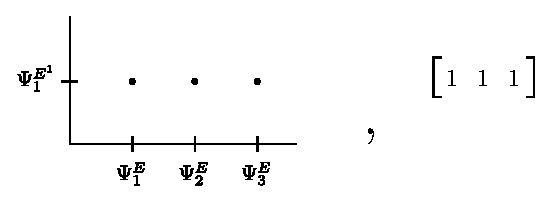
\includegraphics[scale=1.37]{figure/fig4.eps}
\caption{Flat}\label{fig04}
\end{figure}

\newpage
(b) 
\begin{figure}[h]
\centering
\includegraphics[scale=1.3]{figure/fig5.eps}
\caption{Pole}\label{fig05}
\end{figure}

(c)
\begin{figure}[h]
\centering
\includegraphics[scale=1.3]{figure/fig6.eps}
\caption{Grid, Factorable}\label{fig06}
\end{figure}

\newpage

(d)
\begin{figure}[h]
\centering
\includegraphics[scale=1.2]{figure/fig7.eps}
\caption{Steep}\label{fig07}
\end{figure}

(e)
\begin{figure}[h]
\centering
\includegraphics[scale=1]{figure/fig8.eps}
\caption{}\label{fig05}
\end{figure}

\end{example}

\begin{thm}\label{thm-3.3}
It $\overline{\boldsymbol{\psi}}$ is factorable via $E$ Then $| \overline{\boldsymbol{\psi}} \rangle$ is a product vector in the bipartite cut $(E, E')$. In particular, it is so if $\overline{\boldsymbol{\Psi}}$ is flat or a pole via $E$.
\end{thm}

\begin{proof}
It is is immediate from definition that 
\begin{equation}
| \overline{\boldsymbol{\psi}} = \frac{1}{\# \overline{\boldsymbol{\Psi}}} \sum_{\substack{1 \leq j \leq j'}\\ 1 \leq k \leq k'} | \psi^{E}_{j} \rangle \bigotimes | \psi_{k}^{E'} \rangle = \frac{1}{\# \overline{\boldsymbol{\Psi}}}\left(\sum_{j=1}^{j} | \psi_{j}^{E} \rangle\right) \bigotimes \left(\sum_{k=1}^{k'} | \psi_{k}^{E'}\right) \tag{3.20}\label{eq-3.20}
\end{equation}

Hence $| \overline{\boldsymbol{\Psi}}\rangle$ is a product vector in the cut $(E, E')$.

\end{proof}


\begin{subsubsec}\label{subsubsection-3.1.6}

\textbf{Entanglement properties of $\mathbf{| \overline{\boldsymbol{\psi}} \rangle}$ via polynomial representation.} In new of Theorems~\ref{thm-3.1}, \ref{thm-3.3} and intermediary discussion we can confine our attention to the case when $v \geq 4$, $\overline{\bold{\Psi}}$ is decomposable via some  $E$ with $\phi \neq E_{\#} \subset \Gamma_{n}$ and $\Phi~~ \overline{\boldsymbol{\Psi}}$ is not factorable. We will do a little representation here in connection with polynomial representation of $| \overline{\boldsymbol{\Psi}} \rangle$ to streamline the proof of our next Theorem. We will use the notation and terminology above, particularly the lot in \eqref{subsubsection-3.1.5} above.
\end{subsubsec}

\begin{enumerate}[label=(\alph*)]

\item The polynomial representation of the unit vectors $| \Phi_{1} \rangle$, $| \Phi_{2} \rangle$, $| \Phi_{1} \times \Phi_{2} \rangle$  in $\mathcal{H}_{E}$, $\mathcal{H}_{E'}$, $\mathcal{H}$ respectively are given by 
\begin{align*}
F_{\Psi_{1} \times \Psi_{2}} (\boldsymbol{\x}_{E}) & =  2^{-v_{1}/2} \prod_{a\in E \cap A}(\x_{\Psi_{1}(a)}- \x_{a}),~~\\
 &\qquad\qquad\quad F_{\Psi_{1} \times \Psi_{2}} (\boldsymbol{\x}_{E'})= 2^{-v_{2}/2} \prod_{a \in E' \cap A}(\x_{\Psi_{2}(a)}-\x_{a})\\
F_{\Psi_{1} \times \Psi_{2}} (\boldsymbol{\x}) &= 2^{-v/2} \prod_{a \in A} (\x_{\Psi_{1} \times \Psi_{2}(a)} - \x_{a})\\
F_{\Psi_{1} \times \Psi_{2}} (\boldsymbol{\x}) &= F_{\Psi_{1}} (\boldsymbol{\x}_{E})~~ F_{\Psi_{2}}(\boldsymbol{\x}_{E'})\tag{3.21}
\end{align*}

This justifies the rotation $\Psi_{1} \times \Psi_{2}$ set up in \ref{subsubsection-3.1.5} (b) above.

\item For $1 \leq j \leq j'$, let $T_{j} = \left\{k : 1 \leq k \leq k', \Psi_{j}^{E} \times \Psi_{k}^{E'} \in \overline{\boldsymbol{\Psi}}\right\}$, and for $1 \leq k \leq k'$, let $S_{E} = \left\{j : 1 \leq j \leq j', \Psi_{j}^{E} \times \Psi_{K}^{E'} \in  \overline{\boldsymbol{\Psi}}\right\}$. Then all these sets are non-empty  and $\overline{\boldsymbol{\Psi}} = \underset{j=1}{\overset{j'}{\bigcup}} ~~ \underset{R \in T_{j}}{\overset{}\bigcup} \left\{\Psi_{j}^{E} \times \Psi_{K}^{E'}\right\} = \underset{K=1}{\overset{k'}{\bigcup}}~~ \underset{j\in S_{k}}{\overset{}{\bigcup}}\left\{\Psi_{j}^{E} \times \Psi_{K}^{E'} \right\}$.

The unions are all disjoint and $s = \# \overline{\boldsymbol{\Psi}} = \underset{j=1}{\overset{j}{\sum}} \# T_{j} = \underset{k=1}{\overset{R'}{\sum}} \# S_{k}$.

We may express concepts in Definition~\ref{definition-3.2} in terms of $\# T_{j}$ , $\# S_{k}$ for $1 \leq k \leq k'$ For instance, $\overline{\boldsymbol{\Psi}}$ is factorable if and only if $\# T_{j} = k'$ for $1 \leq j \leq j'$ if and only if $\# S_{k} = j'$ for $1 \leq k \leq k'$ if and only $\therefore~ ??? = \# \overline{\boldsymbol{\Psi}} = j'^{k'}$.  

\item For $\Psi \in {\boldsymbol{\Psi}}$ let $p_{\Psi} ({\boldsymbol{\x}}_{E}) = p_{\boldsymbol{\x}_{E}}= 2^{v/2}F_{\Psi/E}({\boldsymbol{\x}}_{E})= \prod\limits_{\substack{a\in E \cap A}}(\x_{\Psi(a)}- \x_{a})$ and $q_{\Psi}({\boldsymbol{\x}}_{E'}) = q_{\Psi/E'}(\boldsymbol{\x}_{E}) = 2^{v_{2}/2} F_{\Psi/E'} ({\boldsymbol{\x}}_{E'}) = \prod\limits_{\substack{a \in E' \cap A}} (\x_{\Psi(a)} - \x_{a})$.

Set 
\begin{equation}
p^{0}_{\Psi}(\boldsymbol{\x}_{E}) = p^{0}_{\Psi/E}(\boldsymbol{\x}_{E}) = \sum_{\phi \neq A_{1_{\neq}} \subset E \cap A}(-1)^{\# A_{1}} {\boldsymbol{\x}^{A_{1}}} {\boldsymbol{\x}^{E \cap B \smallsetminus \Psi(A_{1})}}\tag{3.22}\label{eq-3.22}
\end{equation}
and 
\begin{equation}
q_{\Psi}^{0} (\boldsymbol{\x}_{E'}) = q^{0}_{\Psi/E'}(\boldsymbol{\x}_{E'})= \sum_{\phi \neq A_{2_{\neq}} \subset E' \cap A}(-1)^{\# A_{s}} {\boldsymbol{\x}^{A_{s}}} {\boldsymbol{\x}^{E' \cap B \smallsetminus \Psi(A_{2})}}\tag{3.23}\label{eq-3.23}
\end{equation}
Then
\begin{equation}
p_{\Psi}(\boldsymbol{\x}_{E}) = \boldsymbol{\x}^{E \cap B} + (-1)^{v_{1}} \boldsymbol{\x}^{E \cap A} + p^{0}_{\Psi}(\boldsymbol{\x}_{E})\tag{3.24}
\end{equation}
and
\begin{equation}
q_{\Psi}(\boldsymbol{\x}_{E'}) = \boldsymbol{\x}^{E' \cap B} + (-1)^{v_{2}} \boldsymbol{\x}^{E' \cap A} + q^{0}_{\Psi}(\boldsymbol{\x}_{E'})\tag{3.25}
\end{equation}

\item Let $s= \# \overline{\boldsymbol{\Psi}}$. We set $| \overline{\boldsymbol{\psi}} \rangle = 2^{v/2} \# \overline{\boldsymbol{\psi}} |\overline{\boldsymbol{\psi}} \rangle$. Its $p$ entanglement properties are same as that for $| \overline{\boldsymbol{\psi}} \rangle$.

Its polynomial representation has coefficients as integers and that is convenient to work with.

Indeed,
%~ \begin{equation}
\begin{align*}
F_{\overline{\boldsymbol{\Psi}}}(\boldsymbol{\x}) &= \sum_{\Psi \in \overline{\boldsymbol{\Psi}}} p_{\Psi} (\boldsymbol{\x}_{E})~~ q_{\Psi} (\boldsymbol{\x}_{E'})\\
&= \sum_{\Psi \in \overline{\boldsymbol{\Psi}}} \Bigg((\boldsymbol{\x}^{B}) + (-1)^{v}~~\boldsymbol{\x}^{A} + (-1)^{v_{1}}~~ \boldsymbol{\x}^{E \cap A} ~~\boldsymbol{\x}^{E'\cap B} + (-1)^{v_{2}}~~ \boldsymbol{\x}^{E \cap B}~~ \boldsymbol{\x}^{E' \cap A})\\ 
 &\quad  \left(\boldsymbol{\x}^{E \cap B} + (-1)^{v_{1}}~~ \boldsymbol{\x}^{E \cap A}\right)~~q_{\Psi}^{0} (\boldsymbol{\x}_{E'})  + p_{\Psi}^{0}(\boldsymbol{\x}_{E})~~ \left(\boldsymbol{\x}^{E' \cap B} + (-1)^{v_{2}}~~ \boldsymbol{\x}^{E' \cap A} \right)\\
 &\quad p_{\Psi}^{0}~~ (\boldsymbol{\x}_{E})~~ q_{\Psi}^{0}(\boldsymbol{\x}_{E'}) \Bigg)\\
 & = \# \overline{\boldsymbol{\Psi}} \left(\boldsymbol{\x}^{B} + (-1)^{v} \boldsymbol{\x}^{A} + (-1)^{v_{1}} \boldsymbol{\x}^{E \cap A} \boldsymbol{\x}^{E' \cap B} + (-1)^{v_{2}} \boldsymbol{\x}^{E \cap B} \boldsymbol{\x}^{E' \cap A} \right)\\
 &\quad + \left(\boldsymbol{\x}^{E \cap B} + (-1)^{v_{1}} \boldsymbol{\x}^{E \cap A}\right) \sum_{\Psi \in \overline{\boldsymbol{\Psi}}} q_{\Psi}^{0}(\boldsymbol{\x}_{E'}) + \sum_{\Psi \in \overline{\boldsymbol{\Psi}}} p_{\Psi}^{0}(\boldsymbol{\x}_{E}) \\
 &\hspace{7cm} \left(\boldsymbol{\x}^{E' \cap B} + (-1)^{v_{2}} \boldsymbol{\x}^{E \cap B} \boldsymbol{\x}^{E' \cap A} \right)\\
 & \quad + \sum_{\Psi \in \overline{\boldsymbol{\Psi}}} p_{\Psi}^{0} (\boldsymbol{\x}_{E}) q^{0}_{\Psi} (\boldsymbol{\x}_{E'})\tag{3.26}\label{eq-3.26}
\end{align*}
%~ \end{equation}

\item Consider homogeneous polynomials $p(\boldsymbol{\x}_{E})$ and $q(\boldsymbol{\x}_{E'})$ of degrees $v_{1}$ and $v_{2}$ respectively. They have the form
$p(\boldsymbol{\x}_{E}) = \delta \boldsymbol{\x}^{E \cap A} + \beta\boldsymbol{\x}^{E \cap B} + p_{0}(\boldsymbol{\x}_{E})$ with
\begin{equation}
p_{0}(\boldsymbol{\x_{E}}) = \sum\left\{\delta_{A_{1}, B_{1}} \boldsymbol{\x}^{A_{1}} \boldsymbol{\x}^{E \cap B \smallsetminus B_{1}} : \phi \neq A_{1 \neq} \subset E \cap A, \phi \neq B_{1 \neq} \subset E \cap B, \# A_{1}= \# B_{1}\right\}\tag{3.27}\label{eq-3.27} 
\end{equation}

and $q(\boldsymbol{\x}_{E'}) = \delta^{1} \boldsymbol{\x}^{E' \cap A} + \beta^{1} \boldsymbol{\x}^{E' \cap B} + q_{0}(\boldsymbol{\x}_{E'})$ with
\begin{equation}
q_{0}(\boldsymbol{\x}_{E'}) = \sum \left\{\delta'_{A_{1}, B_{2}} \boldsymbol{\x}^{A_{2}} \boldsymbol{\x}^{E' \cap B \smallsetminus B_{2}} : \phi \neq A_{2 \neq} \subset E' \cap A, \phi \neq B_{2 \neq} \subset E' \cap B, \# A_{2} = \# B_{2}\right\}\tag{3.28}
\end{equation}

where $\delta, \beta, \delta', \delta{'}, \beta_{'}, \delta_{A_{1}, B_{1}}$ are all scalars.

So
\begin{align*}
p(\boldsymbol{\x}_{E}) q (\boldsymbol{\x}_{E'}) &= \delta \delta' \boldsymbol{\x}^{A} + \beta \beta' \boldsymbol{\x}^{B} + \delta \beta' \boldsymbol{\x^{E \cap A}} \boldsymbol{\x}^{E' \cap B} + \delta'\beta \x^{E' \cap A} \boldsymbol{\x}^{E \cap B} +\\
&\quad(\alpha \boldsymbol{\x}^{E \cap A} + \beta \boldsymbol{\x}^{E \cap B}) q_{0}(\boldsymbol{\x}_{E'}) + p_{0}(\x_{E}) (\delta' \boldsymbol{\x}^{E' \cap A} +\beta' \boldsymbol{\x}^{E' \cap B}) +\\
&\quad p_{0}(\boldsymbol{\x}_{E}) q_{0}(\boldsymbol{\x}_{E'})\tag{3.29}
\end{align*}
 
\item We compare (3.26) in (d) and (3.29) in (e) above. 

We obtain that $\widetilde{F}_{\boldsymbol\Psi}(\boldsymbol{\x}) = p(\boldsymbol{\x}_{E}) q(\boldsymbol{\x}_{E'})$ if and only if
\begin{align*}
\beta \beta' &= s = (-1)^{v} \alpha \alpha' = (-1)^{v_{1}} \alpha \beta' = (-1)^{v_{2}} \alpha' \beta\tag{3.30}\label{eq-3.30}\\
\beta q_{0}(\boldsymbol{\x}_{E'}) &= \sum_{\psi \in \boldsymbol{\Psi}} q_{\Psi}^{0}(\boldsymbol{\x}_{E'}) = (-1)^{v_{1}} \alpha q_{0} (\boldsymbol{\x}_{E'})\tag{3.31}\label{eq-3.31}\\
\beta' p_{0}(\boldsymbol{\x}_{E}) &= \sum_{\psi \in \boldsymbol{\Psi}} p^{0}_{\psi} (\boldsymbol{\x}_{E}) = (-1)^{v_{2}} \delta' p_{0} (\boldsymbol{\x})\tag{3.32}\label{eq-3.32}\\
 \text{and}\quad p_{0}(\boldsymbol{\x}_{E}) q_{0}(\boldsymbol{\x}_{E'}) &= \sum_{\psi \in \boldsymbol{\Psi}} p^{0}_{\psi} (\boldsymbol{\x}_{E}) q^{0}_{\psi} (\boldsymbol{\x}_{E'}) \tag{3.33}\label{eq-3.33}
\end{align*}
 
 \item Let us first consider the case when this does happen By (3.30) $\alpha = (-1)^{v_{1}} \beta$, $\alpha' = (-1)^{v_{2}} \beta'$ and $\alpha, \beta, \alpha', \beta'$ are all non-zero.
 
 So we may take $\beta = s$, $\delta = (-1)^{v_{1}} s$, $\beta' = 1$, $\delta' = (-1)^{v_{2}}$ and multiply $p_{0}(\boldsymbol{\x}_{E})$ and $q_{0}(\boldsymbol{\x}_{E'})$ by suitable scalars if the need be and retain the same notation for them. Then~\eqref{eq-3.31} and \eqref{eq-3.32} give $s q_{0}(\boldsymbol{\x}_{E'}) = \sum\limits_{\psi \in \boldsymbol{\Psi}} q_{\psi}^{0} (\boldsymbol{\x}_{E'})$ and $p_{0}(\boldsymbol{\x}_{E}) = \sum\limits_{\psi \in \boldsymbol{\Psi}} p^{0}_{\psi}(\boldsymbol{\x}_{E})$. This turns~\eqref{eq-3.33} into
 \begin{equation}
 \left(\sum_{\psi \in \boldsymbol{\Psi}} p^{0}_{\psi}(\boldsymbol{\x}_{E})\right) \left(\sum_{\psi \in \boldsymbol{\Psi}} q^{0}_{\psi} (\boldsymbol{\x}_{E'})\right) = s \sum_{\psi \in \boldsymbol{\Psi}} p^{0}_{\psi} (\boldsymbol{\x}_{E}) q^{0}_{\psi}(\boldsymbol{\x}_{E'})\tag{3.34}\label{eq-3.34} 
  \end{equation}

For notational convenience, We write $p_{\psi^{E}}^{0} (\boldsymbol{\x}_{E})$ as $p^{0}_{j}(\boldsymbol{\x}_{E})$ and $q^{0}_{\psi_{k}^{E'}} (\boldsymbol{\x}_{E'})$ as $q_{k}^{0}(\boldsymbol{\x}_{E'})$ for $1\leq j \leq j'$, $1\leq k \leq k'$. 

We expand both sides of \eqref{eq-3.34} using (b) above in parts.

\begin{align*}
\text{L.H.S}~~\text{of}~~{\eqref{eq-3.34}} &= \left(\sum_{j=1}^{j'}  \# T_{j} p_{j}^{0}(\boldsymbol{\x}_{E})\right)\left(\sum_{R=1}^{k'} \#S_{k}~ q_{R}^{0}(\boldsymbol{\x}_{E'})\right)\\
&= \sum_{j=1}^{j'} \sum_{k=1}^{k'} \# T_{j} \#S_{k} p_{j}^{0}(\boldsymbol{\x}_{E}) q_{k}^{0}(\boldsymbol{\x}_{E'}).\tag{3.35}\label{eq-3.35}
\end{align*}

Now by (b) above $s= \sum_{k=1}^{k'} \# S_{k} = \sum_{j=1}^{j'} \# T_{j}$.

R.H.S of \eqref{eq-3.34}
\begin{equation}
s\sum_{j=1}^{j'} p_{j}^{0} (\boldsymbol{\x}_{E}) \left(\sum_{l \in T_{j}} q_{l}^{0}(\boldsymbol{\x}_{E'})\right) = s\sum_{k=1}^{k}  \left(\sum_{t \in S_{k}}  p_{T}^{0} (\boldsymbol{\x}_{E})\right) q_{R}^{0} (\boldsymbol{\x}_{E'})\tag{3.36}\label{eq-3.36}
\end{equation}

Equating L.H.S  and R.H.S of~\eqref{eq-3.34}, we obtain
\begin{equation}
\sum_{j=1}^{j'} p_{j}^{0}(\boldsymbol{\x}_{E}) \left(\sum_{l\in T_{j}} (\# T_{j} \# S_{l} -s) q_{l}^{0}(\boldsymbol{\x}_{E'}) + \sum_{\substack{1 \leq k \leq k' \\ k \neq T_{j}}}, \# T_{j} \# S_{k} q_{k}^{0} (\boldsymbol{\x}_{E'}) \right) = 0 \tag{3.37}\label{eq-3.37}
\end{equation}
and
\begin{equation}
\sum_{k=1}^{k'} \left(\sum_{t \in S_{k}} (\# T_{t} \# S_{k} -s) p_{t}^{0}(\boldsymbol{\x}_{E}) +  \sum_{\substack{1 \leq j \leq j' \\ j \notin S_{k}}}, \# T_{j} \# S_{k}  p_{j}^{0}(\boldsymbol{\x}_{E})\right) q_{k}^{0}(\boldsymbol{\x}_{E'}) = 0\tag{3.38}\label{eq-3.38}
\end{equation}

\item Arguments in (g) above can be reversed and , therefor, we call \eqref{eq-3.34}, \eqref{eq-3.37}, \eqref{eq-3.38} Master Equations for $\widetilde{F}_{\boldsymbol{\Psi}}(\boldsymbol{\x})$ to be expressible as product of some polynomials $p(\boldsymbol{\x}_{E})$ and $q(\boldsymbol{\x}_{E'})$. We emphasize that the Master Equations do not involve $p(\boldsymbol{\x}_{E})$ or $q(\boldsymbol{\x}_{E'})$ and in  fact they are determined in an explicit way as explained in (g) above, Moreover, they are equivalent conditions for $| \Psi \rangle$ to be a product vector in the bipartite cut $(E, E')$.
\end{enumerate}


We give easy consequences of the Master equations be fore going to generalities. The spirit of the converse or partial converses of Theorem~\ref{thm-3.3}.

\begin{thm}\label{thm-3.4}
\textbf{Dichotomy}. Consider the following two conditions for $\boldsymbol{\Psi}$ with $\# \boldsymbol{\Psi} \geq 2$.
\begin{enumerate}[label=(\alph*)]

\item Either $\boldsymbol{\Psi}$ is flat or a pole.

\item $| \boldsymbol{\Psi} \rangle$ is genuinely entangled.

\end{enumerate}

If $s=\# \boldsymbol{\Psi}$ is a prime number then one and only one of (a) and (b) holds.

\end{thm}

\begin{proof}
If (a) holds then by Theorem~\ref{thm-3.3}, $| \Psi \rangle$ is not genuinely entangled. So at most one of (a) or (b) can hold.

Now consider the case when (a) does not hold. Let, if possible, (b) not hold. Then $|\boldsymbol{\Psi} \rangle$ is a product vector in some bipartite cut $(E, E')$. By Theorem~\ref{thm-3.1} (ii), and its proof, $\boldsymbol{\Psi}$ is decomposable via $E$ and $F_{\boldsymbol{\Psi}}(\boldsymbol{\x}) = p(\boldsymbol{\x}_{E}) q (\boldsymbol{\x}_{E'})$ for some polynomials $p$ and $q$.

By Master Equation~\ref{eq-3.34}, we have
\begin{equation}
\left(\sum_{\psi \in \boldsymbol{\Psi}} p_{\psi}^{0}(\boldsymbol{\x}_{E})\right) \left(\sum_{\psi \in \boldsymbol{\Psi}} q_{\psi}^{0} (\boldsymbol{\x}_{E'}) \right) = \sum_{\psi \in \boldsymbol{\Psi}} p_{\psi}^{0}(\boldsymbol{\x}_{E}) q_{\psi}^{0}(\boldsymbol{\x}_{E'})\tag{ME}\label{eq-ME}
\end{equation}
 
Consider any $a \in E \cap A$, $a' \in E' \cap A$ and any $\varphi \in \boldsymbol{\Psi}$. Put $b = \varphi(a)$, $b' = \varphi(a')$. Let $U = \left\{\Psi \in \boldsymbol{\Psi} : \varphi \psi(a) = b \right\}$, $V= \left\{\psi \in \boldsymbol{\Psi} : \psi(a) \neq b \right\}$, $W = \left\{\psi \in \boldsymbol{\Psi} : \psi(a) = b, \psi(a') = b'\right\}$,  $u =\# U$, $v = \# V$, $w = \# W$. Then $\varphi \in W \subset U \cap V$. So $1 \leq w \leq \min \{u, v\}$. Because $\boldsymbol{\Psi}$ is neither flat nor a pole, we have $V \subset_{\neq} \boldsymbol{\Psi}$, $U \subset_{\#} \boldsymbol{\Psi}$. So $u < s$, $v < s$.
 
The co-efficient of $\boldsymbol{\x}^{\{a\}}$ $\boldsymbol{\x}^{E \cap B \smallsetminus \{b\}}$ in $\sum_{\psi \in \boldsymbol{\Psi}} p_{\psi}^{0}(\boldsymbol{\x}_{E})$ is -u and that of $\boldsymbol{\x}^{\{a'\}}$ $\boldsymbol{\x}^{E' \cap B \smallsetminus \{b'\}}$ in $\sum_{\psi \in \boldsymbol{\Psi}} q_{\psi}^{0}(\x_{E'})$ is $-v$. So the co-efficient of $\boldsymbol{\x}^{\{a, a'\}}$ $\boldsymbol{\x}^{B \smallsetminus \{b, b'\}}$ in the L.H.S of \eqref{eq-ME} is $uv$. On the other hand, the coefficient of $\boldsymbol{\x}^{\{a, a'\}}$ $\boldsymbol{\x}^{B \smallsetminus \{b, b'\}}$ on  The R.H.S of \eqref{eq-ME} is $sw$. So we have the equation 
\begin{equation}
uv=sw \tag{3.39}\label{eq-3.39}
\end{equation}

Now $1 \leq u < s$ and $1 \leq v < s$. So $s$ cannot be a factor of $u$ or $v$. So if $s$ is a prime, then $s$ cannot be a factor of $uv$. This contradicts~\eqref{eq-3.39}. Hence $| \boldsymbol{\Psi} \rangle$ is genuinely entangled, i.e., (b) holds.
 
\end{proof}

\begin{thm}\label{thm-3.5}
Let $\boldsymbol{\Psi}$ be decomposable via $E$ and $\{p_{j}^{0}(\boldsymbol{\x}_{E}) 1 \leq j \leq j'\}$ and $\{q_{k}^{0} (\boldsymbol{\x}_{E'}) : 1 \leq k \leq k'\}$ and other symbols be as in ~\eqref{subsubsection-3.1.6} above. Suppose that both these systems are linearly independent. If $| \boldsymbol{\Psi} \rangle$ is a product vector in the biparlite cut $(E, E')$ the $\boldsymbol{\Psi}$ is factorable via $E$.
\end{thm}

\begin{proof}
By the Master Equation \eqref{eq-3.37}, the linear independence of $\left\{p_{j}^{0} (\boldsymbol{\x}_{E}) : 1 \leq j \leq j'\right\}$ forces the following. For $1 \leq j \leq j'$,  
\begin{equation}
\sum\limits_{l\in T_{j}} (\# T_{j} \# S_{l}-s) q_{l}^{0}(\boldsymbol{\x}_{E'}) + \sum_{1 \leq k \leq k'}, \# T_{j} \# S_{k} q_{k}^{0}(\boldsymbol{\x}_{E'}) = 0\tag{3.40}\label{eq-3.40} 
\end{equation}

But $\left\{q_{k}^{0}(\boldsymbol{\x}_{E}): 1 \leq k \leq k' \right\}$ is linearly independent and $\# T_{j} \neq 0 \neq \# S_{k}$ for $1 \leq j \leq j'$, $1 \leq k \leq k'$. So $T_{j} = \left\{k : 1 \leq k \leq k'\right\}$ for $1 \leq j \leq j'$.

This gives that $\boldsymbol{\Psi}$ is factorable via $E$.
\end{proof}

\begin{example}\label{example-3.3}
We give instance of $\boldsymbol{\Psi}$ for which the conditions of linear independence as in Theorem~\ref{thm-3.5} above holds. 

(a) Let $v=5$, $E = \{1,2,3,4,5,6\}$, $E' = \{7,8,9,10\}$.

Let $\boldsymbol{\Psi}$ consist of the four coverings $\psi (j), j = 1,2,3,4$ as in Figure~\ref{fig09}.
\end{example}

\begin{figure}[h]
\centering
\includegraphics[scale=1.1]{figure/figures/fig9.eps}
\caption{}\label{fig09}
\end{figure}

Then 
\begin{align*}
\boldsymbol{\Psi}_{E} &= \left\{\psi^{(1)}/E , \psi^{(2)}/E, \psi^{(3)}/E\right\},\\
\boldsymbol{\Psi}_{E'} & = \left\{\psi^{(1)}/E' , \psi^{(2)}/E'\right\}.
\end{align*}



The grid is given by Figure~\ref{fig10} which shows that $\boldsymbol{\Psi}$ is not factorable. Indeed $j' =3$, $k'=2$ whereas $s = 4$.

\newpage

\begin{figure}[h]
\centering
\includegraphics[scale=1.1]{figure/figures/fig10.eps}
\caption{}\label{fig10}
\end{figure}

 (c) For tuples $\boldsymbol{\lambda} = (\lambda_{1}, \lambda_{2}, \lambda_{3})$, $\mu =(\mu_{1}, \mu_{2})$ of consider the polynomials $p^{\boldsymbol{\lambda}}{\boldsymbol{\x}_{E}}) = \sum\limits_{j=1}^{3} \lambda_{j} \cdot p_{j}^{0} (\boldsymbol{\x}_{E})$ and $q^{\mu}(\boldsymbol{\x}_{E'}) = \sum\limits_{\mu =1}^{2} \mu_{k} q_{k}^{0} (\boldsymbol{\x}_{E'})$. Then the coefficient of $\x_{1}~ \x_{4}~\x_{6} = \boldsymbol{\x}^{\{1\}} \boldsymbol{\x}^{\{4,6\}}$, $\x_{1}~ \x_{2} ~\x_{6} = \x^{\{1\}} \boldsymbol{\x}^{\{2,6\}}$, $\x_{1} \x_{2} \x_{4} = \x^{\{1\}} \boldsymbol{\x}^{\{2,4\}}$ in $p^{\boldsymbol{\lambda}}(\boldsymbol{\x}_{E})$ are $\lambda_{1}, \lambda_{2}, \lambda_{3}$ respectively. So $p^{\boldsymbol{\lambda}}(\boldsymbol{\x}_{E}) =0$ if and only if $\lambda_{1} = 0 = \lambda_{2} = \lambda_{3}$. Hence $\{p_{j}^{0}(\boldsymbol{\x}_{E}), j = 1, 2, 3\}$  is linearly independent. On the other hand, the coefficients of $\x_{7} \x_{10} = \boldsymbol{\x}^{\{7\}} \boldsymbol{\x}^{\{10\}}$ and $\x_{7} \x_{8} = \boldsymbol{\x}^{\{7\}} \boldsymbol{\x}^{\{8\}}$ in $q^{\boldsymbol{\mu}}(\boldsymbol{\x}_{E'})$ are $\mu_{1}$ and $\mu_{2}$ respectively. So $q^{\boldsymbol{\mu}} (\boldsymbol{\x}_{E'})$ is $0$ if and only ???????????? Hence $\{q_{k}^{0}(\boldsymbol{\x}_{E'}): k = 1,2\}$ is linearly independent. ????????? that $| \boldsymbol{\Psi} \rangle$ is not ????
 
 But $\boldsymbol{\Psi}$ is not decomposable via any other bipartite cut. So $| \boldsymbol{\Psi} \rangle$ is genuinely entangled.
 
 This motivates our next definition and result.
 
\begin{definition}\label{definition-3.3}
Let $\boldsymbol{\Psi}$ be as set of coverings of $\Gamma_{n}$ with $\# \boldsymbol{\Psi} \geq 2$.
\end{definition}

\begin{enumerate}[label = (\roman*)]
 \item Suppose that $\boldsymbol{\Psi}$ is decomposable via some with $E$ with $\phi  \neq E \subset_{\neq} \Gamma_{n}$. $\boldsymbol{\Psi}$ will. be said to be \textbf{independent via $\boldsymbol{E}$} if $ \boldsymbol{\Psi}_{E} = \left\{\psi_{j}^{E} : 1 \leq j \leq j' \right\}$ and $\boldsymbol{\Psi}_{E'} = \left\{\psi_{k}^{E'} : 1 \leq k \leq k' \right\}$  satisfy the following conditions.
\begin{enumerate}[label = (\alph*)]
\item For each $j, 1 \leq j \leq j'$ there exists $\phi \neq A^{E}_{j} \subset_{\neq} E \cap A$, $\phi \neq B_{j}^{E} \subset_{\neq} E \cap B$ such that $\left\{t : 1 \leq t \leq j', \psi_{t}^{E} (A_{j}^{E}) = B_{j}^{E}\right\} = \left\{j\right\}$.

\item For each $k$, $1 \leq k \leq k'$, there exists $\phi \neq A_{j}^{E'} \subset_{\neq} E' \cap A$, $\phi\neq B_{k}^{E'} \subset_{\neq} E' \cap B $ such that $\left\{ u : 1 \leq u \leq k' : \psi_{u}^{E'} (A_{k}^{E'} = B_{k}^{E'})\right\} = \{k\}$.

In other words, $\boldsymbol{\x}^{A_{j}^{E}}$ $\boldsymbol{\x}^{E \cap B \smallsetminus B^{E}_{j}}$ does occur in and only in $p_{j}^{0} (\boldsymbol{\x}_{E})$ and $\boldsymbol{\x}^{A_{k}^{E'}}$ $\boldsymbol{\x}^{E' \cap B \smallsetminus B_{k}^{E'}}$ does occur in and only in $q_{k}^{0}(\boldsymbol{\x}_{E'})$.
\end{enumerate}

\item Suppose that neither flat nor a pole. $\boldsymbol{\Psi}$ be called \textbf{independent} if it is independents via $E$ for any $E$ via which $\boldsymbol{\Psi}$  is not decomposable then we note that if $\boldsymbol{\Psi}$ is not decomposable then $\boldsymbol{\Psi}$ is independent by this definition. On the other hand of $\boldsymbol{\x}$ is flat or a pole, then $\boldsymbol{\Psi}$ is not independent by this definition.

\end{enumerate}

\begin{thm}\label{thm-3.6}
Suppose that $\boldsymbol{\Psi}$ is independent. Then $| \boldsymbol{\Psi} \rangle$ is genuinely entangled if and only if $\boldsymbol{\Psi}$ is not factorable.
\end{thm}

\begin{proof}
In view of Theorem~\ref{thm-3.3} if $| \boldsymbol{\Psi} \rangle$ is genuinely entangled then $\boldsymbol{\Psi}$ in not factorable. Now suppose that $\boldsymbol{\Psi}$ is not factorable. Let, if possible, $| \boldsymbol{\Psi} \rangle$ be not genuinely entangled. Then $| \boldsymbol{\Psi} \rangle$ is a 
product vector in some biparlite cut, say, $(E, E')$. Then by Theorem~\ref{thm-3.1} (ii) $\boldsymbol{\Psi}$ is decomposable via $E$. Because $\boldsymbol{\Psi}$ is independent we have that $\boldsymbol{\Psi}$ is independent via $E$. The arguments in Example~\ref{example-3.3} (c) above can be suitably modified to give that $\left\{p_{j}^{0}(\boldsymbol{\x}_{E}) : 1 \leq j \leq j' \right\}$ and $\left\{q_{k}^{0} (\boldsymbol{\x}_{E'})  : 1 \leq k \leq k'\right\}$ are both linearly independent. Indeea let if possible $p^{\lambda}(\boldsymbol{\x}_{E}) = \sum\limits_{j=1}^{j} \lambda_{j} p_{j}(\boldsymbol{\x}_{E}) = 0$ for some triple $\boldsymbol{\lambda} = (\lambda_{j})^{j'}_{j=1}$ of scalars. For $1 \leq j \leq j_{1}, $ the coefficient of $\boldsymbol{\x}^{A_{j}^{E}}$ $\boldsymbol{\x}^{E \cap B \smallsetminus} B_{j}^{E}$ in $p^{\boldsymbol{\lambda}} (\boldsymbol{\x}_{E})$ is $(-1) \# A_{j}~ \lambda_{j}$. So $\lambda_{j} = 0$ for $1 \leq j \leq j'$, similarly we can prove that $\left\{q_{k}^{0}(\boldsymbol{\x}_{E'}) : 1 \leq k \leq k' \right\}$ is linearly independent. By Theorem~\ref{thm-3.5}, $\boldsymbol{\Psi}$ is factorable via $E$, a contradiction.
  

\end{proof}


 
\end{document}
